% Options for packages loaded elsewhere
\PassOptionsToPackage{unicode}{hyperref}
\PassOptionsToPackage{hyphens}{url}
\PassOptionsToPackage{dvipsnames,svgnames,x11names}{xcolor}
%
\documentclass[
  letterpaper,
  DIV=11,
  numbers=noendperiod]{scrartcl}

\usepackage{amsmath,amssymb}
\usepackage{iftex}
\ifPDFTeX
  \usepackage[T1]{fontenc}
  \usepackage[utf8]{inputenc}
  \usepackage{textcomp} % provide euro and other symbols
\else % if luatex or xetex
  \usepackage{unicode-math}
  \defaultfontfeatures{Scale=MatchLowercase}
  \defaultfontfeatures[\rmfamily]{Ligatures=TeX,Scale=1}
\fi
\usepackage{lmodern}
\ifPDFTeX\else  
    % xetex/luatex font selection
\fi
% Use upquote if available, for straight quotes in verbatim environments
\IfFileExists{upquote.sty}{\usepackage{upquote}}{}
\IfFileExists{microtype.sty}{% use microtype if available
  \usepackage[]{microtype}
  \UseMicrotypeSet[protrusion]{basicmath} % disable protrusion for tt fonts
}{}
\makeatletter
\@ifundefined{KOMAClassName}{% if non-KOMA class
  \IfFileExists{parskip.sty}{%
    \usepackage{parskip}
  }{% else
    \setlength{\parindent}{0pt}
    \setlength{\parskip}{6pt plus 2pt minus 1pt}}
}{% if KOMA class
  \KOMAoptions{parskip=half}}
\makeatother
\usepackage{xcolor}
\setlength{\emergencystretch}{3em} % prevent overfull lines
\setcounter{secnumdepth}{-\maxdimen} % remove section numbering
% Make \paragraph and \subparagraph free-standing
\ifx\paragraph\undefined\else
  \let\oldparagraph\paragraph
  \renewcommand{\paragraph}[1]{\oldparagraph{#1}\mbox{}}
\fi
\ifx\subparagraph\undefined\else
  \let\oldsubparagraph\subparagraph
  \renewcommand{\subparagraph}[1]{\oldsubparagraph{#1}\mbox{}}
\fi

\usepackage{color}
\usepackage{fancyvrb}
\newcommand{\VerbBar}{|}
\newcommand{\VERB}{\Verb[commandchars=\\\{\}]}
\DefineVerbatimEnvironment{Highlighting}{Verbatim}{commandchars=\\\{\}}
% Add ',fontsize=\small' for more characters per line
\usepackage{framed}
\definecolor{shadecolor}{RGB}{241,243,245}
\newenvironment{Shaded}{\begin{snugshade}}{\end{snugshade}}
\newcommand{\AlertTok}[1]{\textcolor[rgb]{0.68,0.00,0.00}{#1}}
\newcommand{\AnnotationTok}[1]{\textcolor[rgb]{0.37,0.37,0.37}{#1}}
\newcommand{\AttributeTok}[1]{\textcolor[rgb]{0.40,0.45,0.13}{#1}}
\newcommand{\BaseNTok}[1]{\textcolor[rgb]{0.68,0.00,0.00}{#1}}
\newcommand{\BuiltInTok}[1]{\textcolor[rgb]{0.00,0.23,0.31}{#1}}
\newcommand{\CharTok}[1]{\textcolor[rgb]{0.13,0.47,0.30}{#1}}
\newcommand{\CommentTok}[1]{\textcolor[rgb]{0.37,0.37,0.37}{#1}}
\newcommand{\CommentVarTok}[1]{\textcolor[rgb]{0.37,0.37,0.37}{\textit{#1}}}
\newcommand{\ConstantTok}[1]{\textcolor[rgb]{0.56,0.35,0.01}{#1}}
\newcommand{\ControlFlowTok}[1]{\textcolor[rgb]{0.00,0.23,0.31}{#1}}
\newcommand{\DataTypeTok}[1]{\textcolor[rgb]{0.68,0.00,0.00}{#1}}
\newcommand{\DecValTok}[1]{\textcolor[rgb]{0.68,0.00,0.00}{#1}}
\newcommand{\DocumentationTok}[1]{\textcolor[rgb]{0.37,0.37,0.37}{\textit{#1}}}
\newcommand{\ErrorTok}[1]{\textcolor[rgb]{0.68,0.00,0.00}{#1}}
\newcommand{\ExtensionTok}[1]{\textcolor[rgb]{0.00,0.23,0.31}{#1}}
\newcommand{\FloatTok}[1]{\textcolor[rgb]{0.68,0.00,0.00}{#1}}
\newcommand{\FunctionTok}[1]{\textcolor[rgb]{0.28,0.35,0.67}{#1}}
\newcommand{\ImportTok}[1]{\textcolor[rgb]{0.00,0.46,0.62}{#1}}
\newcommand{\InformationTok}[1]{\textcolor[rgb]{0.37,0.37,0.37}{#1}}
\newcommand{\KeywordTok}[1]{\textcolor[rgb]{0.00,0.23,0.31}{#1}}
\newcommand{\NormalTok}[1]{\textcolor[rgb]{0.00,0.23,0.31}{#1}}
\newcommand{\OperatorTok}[1]{\textcolor[rgb]{0.37,0.37,0.37}{#1}}
\newcommand{\OtherTok}[1]{\textcolor[rgb]{0.00,0.23,0.31}{#1}}
\newcommand{\PreprocessorTok}[1]{\textcolor[rgb]{0.68,0.00,0.00}{#1}}
\newcommand{\RegionMarkerTok}[1]{\textcolor[rgb]{0.00,0.23,0.31}{#1}}
\newcommand{\SpecialCharTok}[1]{\textcolor[rgb]{0.37,0.37,0.37}{#1}}
\newcommand{\SpecialStringTok}[1]{\textcolor[rgb]{0.13,0.47,0.30}{#1}}
\newcommand{\StringTok}[1]{\textcolor[rgb]{0.13,0.47,0.30}{#1}}
\newcommand{\VariableTok}[1]{\textcolor[rgb]{0.07,0.07,0.07}{#1}}
\newcommand{\VerbatimStringTok}[1]{\textcolor[rgb]{0.13,0.47,0.30}{#1}}
\newcommand{\WarningTok}[1]{\textcolor[rgb]{0.37,0.37,0.37}{\textit{#1}}}

\providecommand{\tightlist}{%
  \setlength{\itemsep}{0pt}\setlength{\parskip}{0pt}}\usepackage{longtable,booktabs,array}
\usepackage{calc} % for calculating minipage widths
% Correct order of tables after \paragraph or \subparagraph
\usepackage{etoolbox}
\makeatletter
\patchcmd\longtable{\par}{\if@noskipsec\mbox{}\fi\par}{}{}
\makeatother
% Allow footnotes in longtable head/foot
\IfFileExists{footnotehyper.sty}{\usepackage{footnotehyper}}{\usepackage{footnote}}
\makesavenoteenv{longtable}
\usepackage{graphicx}
\makeatletter
\def\maxwidth{\ifdim\Gin@nat@width>\linewidth\linewidth\else\Gin@nat@width\fi}
\def\maxheight{\ifdim\Gin@nat@height>\textheight\textheight\else\Gin@nat@height\fi}
\makeatother
% Scale images if necessary, so that they will not overflow the page
% margins by default, and it is still possible to overwrite the defaults
% using explicit options in \includegraphics[width, height, ...]{}
\setkeys{Gin}{width=\maxwidth,height=\maxheight,keepaspectratio}
% Set default figure placement to htbp
\makeatletter
\def\fps@figure{htbp}
\makeatother
\newlength{\cslhangindent}
\setlength{\cslhangindent}{1.5em}
\newlength{\csllabelwidth}
\setlength{\csllabelwidth}{3em}
\newlength{\cslentryspacingunit} % times entry-spacing
\setlength{\cslentryspacingunit}{\parskip}
\newenvironment{CSLReferences}[2] % #1 hanging-ident, #2 entry spacing
 {% don't indent paragraphs
  \setlength{\parindent}{0pt}
  % turn on hanging indent if param 1 is 1
  \ifodd #1
  \let\oldpar\par
  \def\par{\hangindent=\cslhangindent\oldpar}
  \fi
  % set entry spacing
  \setlength{\parskip}{#2\cslentryspacingunit}
 }%
 {}
\usepackage{calc}
\newcommand{\CSLBlock}[1]{#1\hfill\break}
\newcommand{\CSLLeftMargin}[1]{\parbox[t]{\csllabelwidth}{#1}}
\newcommand{\CSLRightInline}[1]{\parbox[t]{\linewidth - \csllabelwidth}{#1}\break}
\newcommand{\CSLIndent}[1]{\hspace{\cslhangindent}#1}

\KOMAoption{captions}{tableheading}
\makeatletter
\makeatother
\makeatletter
\makeatother
\makeatletter
\@ifpackageloaded{caption}{}{\usepackage{caption}}
\AtBeginDocument{%
\ifdefined\contentsname
  \renewcommand*\contentsname{Table of contents}
\else
  \newcommand\contentsname{Table of contents}
\fi
\ifdefined\listfigurename
  \renewcommand*\listfigurename{List of Figures}
\else
  \newcommand\listfigurename{List of Figures}
\fi
\ifdefined\listtablename
  \renewcommand*\listtablename{List of Tables}
\else
  \newcommand\listtablename{List of Tables}
\fi
\ifdefined\figurename
  \renewcommand*\figurename{Figure}
\else
  \newcommand\figurename{Figure}
\fi
\ifdefined\tablename
  \renewcommand*\tablename{Table}
\else
  \newcommand\tablename{Table}
\fi
}
\@ifpackageloaded{float}{}{\usepackage{float}}
\floatstyle{ruled}
\@ifundefined{c@chapter}{\newfloat{codelisting}{h}{lop}}{\newfloat{codelisting}{h}{lop}[chapter]}
\floatname{codelisting}{Listing}
\newcommand*\listoflistings{\listof{codelisting}{List of Listings}}
\makeatother
\makeatletter
\@ifpackageloaded{caption}{}{\usepackage{caption}}
\@ifpackageloaded{subcaption}{}{\usepackage{subcaption}}
\makeatother
\makeatletter
\@ifpackageloaded{tcolorbox}{}{\usepackage[skins,breakable]{tcolorbox}}
\makeatother
\makeatletter
\@ifundefined{shadecolor}{\definecolor{shadecolor}{rgb}{.97, .97, .97}}
\makeatother
\makeatletter
\makeatother
\makeatletter
\makeatother
\ifLuaTeX
  \usepackage{selnolig}  % disable illegal ligatures
\fi
\IfFileExists{bookmark.sty}{\usepackage{bookmark}}{\usepackage{hyperref}}
\IfFileExists{xurl.sty}{\usepackage{xurl}}{} % add URL line breaks if available
\urlstyle{same} % disable monospaced font for URLs
\hypersetup{
  pdftitle={Lesson 3: Likelihood-based inference for POMP models},
  pdfauthor={Qianying (Ruby) Lin; Spencer J. Fox; Zian (Larry) Zhuang},
  colorlinks=true,
  linkcolor={blue},
  filecolor={Maroon},
  citecolor={Blue},
  urlcolor={Blue},
  pdfcreator={LaTeX via pandoc}}

\title{Lesson 3: Likelihood-based inference for POMP models}
\author{Qianying (Ruby) Lin \and Spencer J. Fox \and Zian (Larry)
Zhuang}
\date{}

\begin{document}
\maketitle
\ifdefined\Shaded\renewenvironment{Shaded}{\begin{tcolorbox}[breakable, enhanced, interior hidden, sharp corners, boxrule=0pt, borderline west={3pt}{0pt}{shadecolor}, frame hidden]}{\end{tcolorbox}}\fi

\hypertarget{introduction}{%
\section{Introduction}\label{introduction}}

\hypertarget{objectives}{%
\subsection{Objectives}\label{objectives}}

Students completing this lesson will:

\begin{enumerate}
\def\labelenumi{\arabic{enumi}.}
\tightlist
\item
  Gain an understanding of the nature of the problem of likelihood
  computation for POMP models.
\item
  Be able to explain the simplest particle filter algorithm.
\item
  Gain experience in the visualization and exploration of likelihood
  surfaces.
\item
  Be able to explain the tools of likelihood-based statistical inference
  that become available given numerical accessibility of the likelihood
  function.
\end{enumerate}

\hypertarget{overview}{%
\subsection{Overview}\label{overview}}

A general framework of epidemiological inference includes three layers:

\begin{itemize}
\tightlist
\item
  The input: a model of interest and the given data
\item
  A method for inference
\item
  Inferences include estimation, uncertainty, prediction and forecast,
  and model selection.
\end{itemize}

\begin{center}
  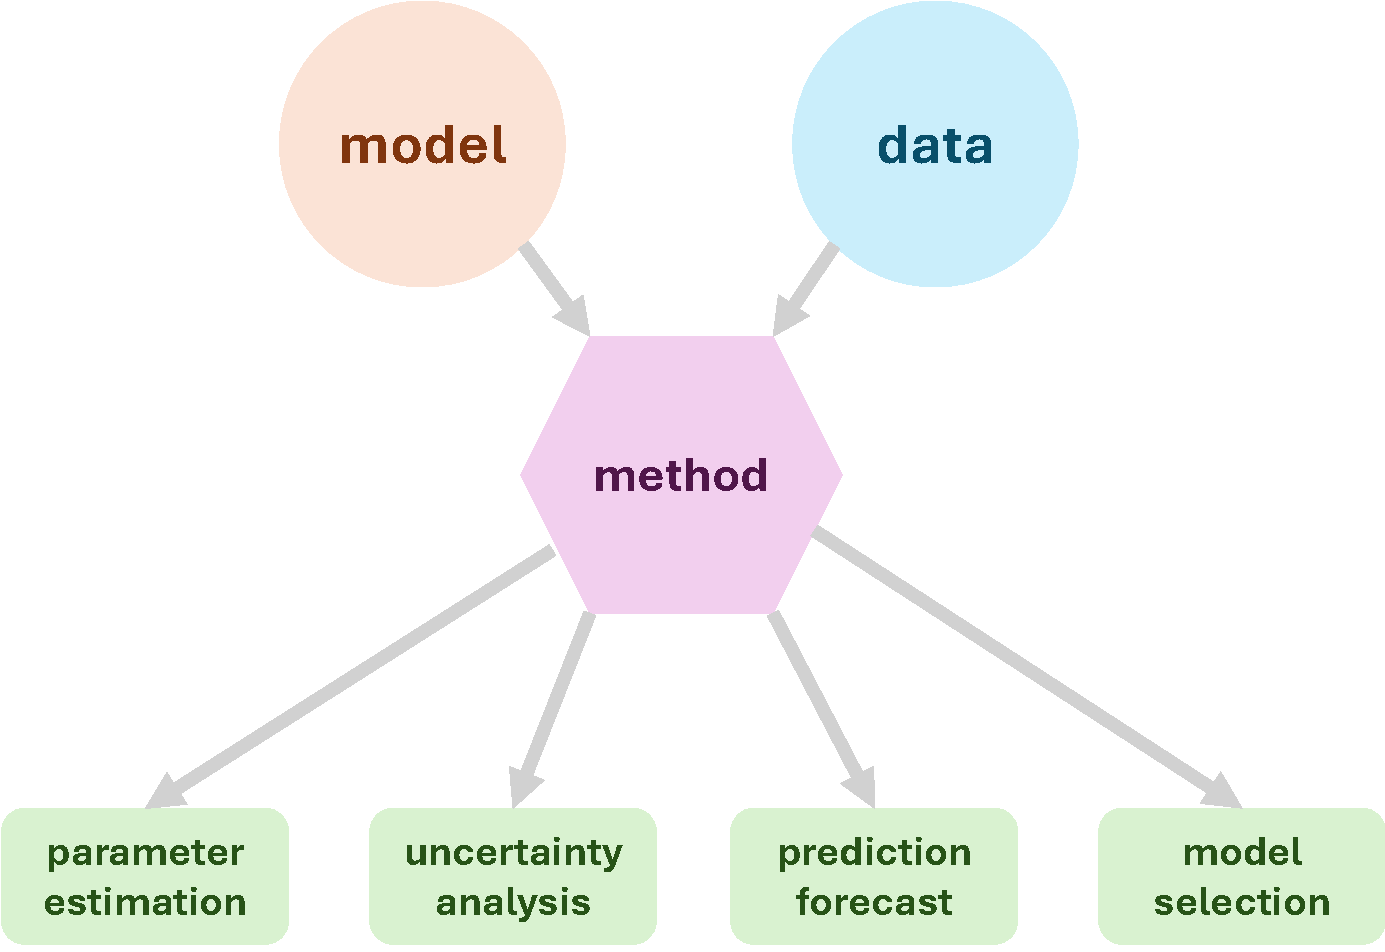
\includegraphics[height=4.5cm]{../graphics/lec3_overview}
\end{center}

\framebreak

Methods for inference can be categorized into three groups:

\begin{itemize}
\tightlist
\item
  Optimization-based: minimize a cost function (e.g., SSE, MSE, MAE)
  that measures the difference between observed data and model
  predictions
\item
  Likelihood-based: maximize a likelihood function, which represents the
  probability of observing the given data given the parameters
\item
  Summary Statistics-based: use a set of features of the data instead of
  the full set of data
\end{itemize}

In this lesson, we focus on the likelihood-based method because

\begin{itemize}
\tightlist
\item
  it fits for stochastic models and
\item
  it incorporates all data (i.e., full-information).
\end{itemize}

\hypertarget{the-likelihood-function}{%
\section{The likelihood function}\label{the-likelihood-function}}

\hypertarget{general-considerations}{%
\section{General considerations}\label{general-considerations}}

\hypertarget{the-likelihood}{%
\subsection{The likelihood}\label{the-likelihood}}

\begin{itemize}
\tightlist
\item
  The basis for modern frequentist, Bayesian, and information-theoretic
  inference.
\item
  Method of maximum likelihood introduced by Fisher (1922).
\item
  The likelihood function itself is a representation of the what the
  data have to say about the parameters.
\item
  A good general reference on likelihood is by Pawitan (2001).
\end{itemize}

\framebreak

\begin{itemize}
\tightlist
\item
  Goal: fit the model to the data and conduct statistical inferences,
  such as parameter estimation.
\item
  The likelihood, thus, can be considered as a metric to assess the
  \emph{goodness} of the proposed parameters.
\item
  By exploring the space of parameters, we can eventually obtain the
  maximum likelihood estimator (MLE).
\end{itemize}

\begin{center}
  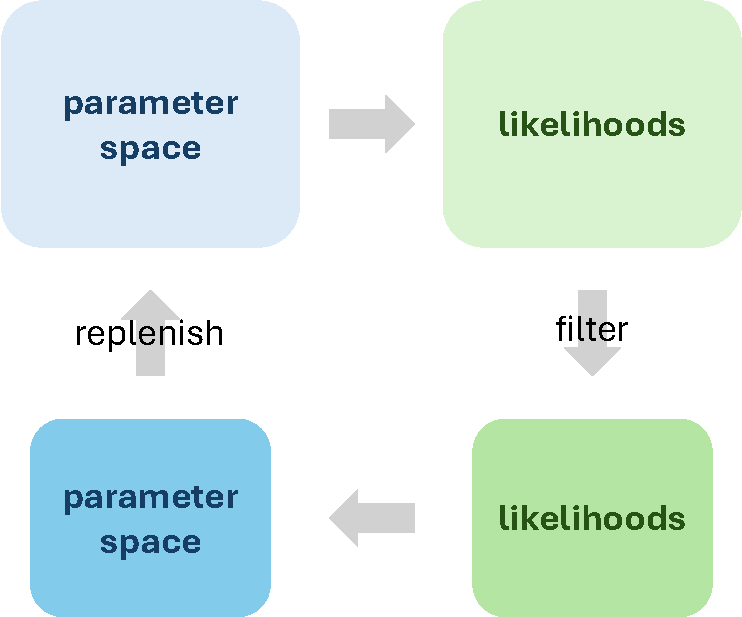
\includegraphics[height=4.5cm]{../graphics/lec3_procedure}
\end{center}

\vfill

Thus, the objective of this lesson is to discuss how we compute the
likelihood given a model of interest with a proposed set of parameters
in both theory and in \texttt{pomp}.

\hypertarget{definition-of-the-likelihood-function}{%
\subsection{Definition of the likelihood
function}\label{definition-of-the-likelihood-function}}

\begin{itemize}
\tightlist
\item
  Notations:

  \begin{itemize}
  \tightlist
  \item
    \(y_{1:N}^*\): the data, a sequence of \(N\) observations
  \item
    \(f_{Y_{1:N}}(y_{1:N};\theta)\): the statistical model, a
    probability distribution for each value of a parameter vector
    \(\theta\)
  \item
    \(Y_{1:N} \sim f_{Y_{1:N}}(y_{1:N};\theta)\): a random variable
    drawn from distribution \(f_{Y_{1:N}}(y_{1:N};\theta)\)
  \end{itemize}
\item
  The likelihood function is
  \[\lik(\theta) = f_{Y_{1:N}}(y^*_{1:N};\theta),\] the density function
  evaluated at the data.
\item
  It is often convenient to work with the log-likelihood function,
  \[\loglik(\theta)= \log \lik(\theta) = \log f_{Y_{1:N}}(y^*_{1:N};\theta).\]
\end{itemize}

\hypertarget{a-simulator-is-implicitly-a-statistical-model}{%
\subsection{A simulator is implicitly a statistical
model}\label{a-simulator-is-implicitly-a-statistical-model}}

\begin{itemize}
\tightlist
\item
  \(f_{Y_{1:N}}(y_{1:N};\theta)\) is simple and with an explicit
  expression:

  \begin{itemize}
  \tightlist
  \item
    the simulation of \(Y_{1:N}\) is direct, e.g., \(Y_k \sim N(0,1)\)
    for \(k=1,\dots,N\)
  \item
    the likelihood function is explicit
  \end{itemize}
\item
  \(f_{Y_{1:N}}(y_{1:N};\theta)\) is complex or even without an explicit
  expression:

  \begin{itemize}
  \tightlist
  \item
    the simulation of \(Y_{1:N}\), given the underlying dynamical model,
    is a bit more complex but convenient
  \item
    the likelihood function exists with a complicated expression or even
    without an explicit expression
  \end{itemize}
\end{itemize}

Thus, we can develop numerical methods to compute the complex or
implicit likelihood functions!

\hypertarget{likelihood-of-a-pomp-model}{%
\section{Likelihood of a POMP model}\label{likelihood-of-a-pomp-model}}

\hypertarget{the-likelihood-for-a-pomp-model}{%
\subsection{The likelihood for a POMP
model}\label{the-likelihood-for-a-pomp-model}}

Recall the following schematic diagram, showing dependence among
variables in a POMP model.

\begin{center}
    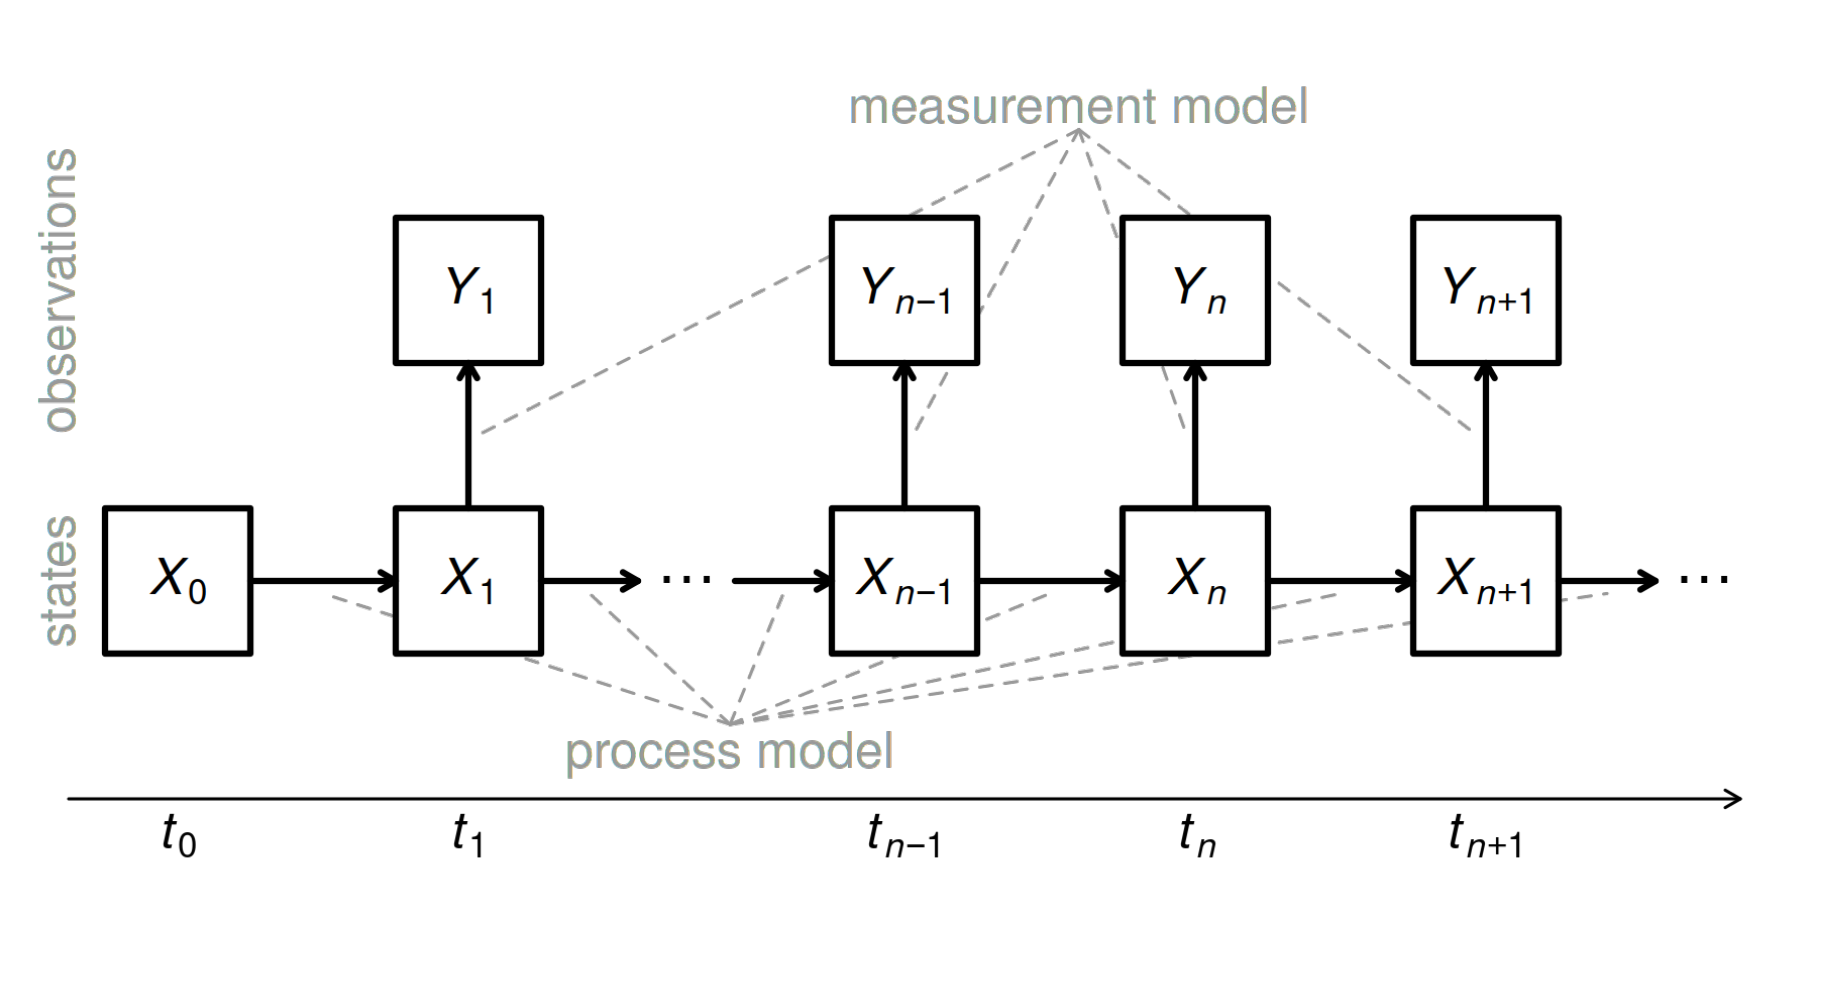
\includegraphics[height=5.5cm]{../graphics/lec3ll.png}
  \end{center}

\framebreak

Recall the following definitions and properties:

\begin{itemize}
\item
  \textbf{Measurements}: \(Y_n\), at time \(t_n\) depend on the latent
  process, \(X_n\), at that time.
\item
  \textbf{The Markov property}: latent process variables depend on their
  value at the previous timestep.

  \begin{enumerate}
  \def\labelenumi{\arabic{enumi}.}
  \tightlist
  \item
    The distribution of the state \(X_{n+1}\), conditional on \(X_{n}\),
    is independent of the values of \(X_{k}\), \(k<n\) and \(Y_{k}\),
    \(k\le n\).
  \item
    The distribution of the measurement \(Y_{n}\), conditional on
    \(X_{n}\), is independent of all other variables.
  \end{enumerate}
\item
  \textbf{The latent process}: \(X(t)\), may be defined at all times,
  but we are particularly interested in its value at observation times.
  Therefore, we write \[X_n=X(t_n).\]

  \begin{itemize}
  \tightlist
  \item
    We write collections of random variables using the notation
    \(X_{0:N}=(X_0,\dots,X_N)\).
  \end{itemize}
\item
  \textbf{The one-step transition density}:
  \(f_{X_n|X_{n-1}}(x_n|x_{n-1};\theta)\), together with the measurement
  density, \(f_{Y_n|X_n}(y_n|x_n;\theta)\) and the initial density,
  \(f_{X_0}(x_0;\theta)\), specify the entire joint density via

  \[
    \begin{split}
            &f_{X_{0:N},Y_{1:N}}(x_{0:N},y_{1:N};\theta)\\
            & \qquad = f_{X_0}(x_0;\theta)\,\prod_{n=1}^N\!f_{X_n | X_{n-1}}(x_n|x_{n-1};\theta)\,f_{Y_n|X_n}(y_n|x_n;\theta).
    \end{split}
  \]
\item
  \textbf{The marginal density for sequence of measurements}:
  \(Y_{1:N}\), evaluated at the data, \(y_{1:N}^*\), is \[
    \lik(\theta) = f_{Y_{1:N}}(y^*_{1:N};\theta)=\int\!f_{X_{0:N},Y_{1:N}}(x_{0:N},y^*_{1:N};\theta)\, dx_{0:N}.
  \]
\end{itemize}

\hypertarget{special-case-deterministic-latent-process}{%
\subsection{Special case: deterministic latent
process}\label{special-case-deterministic-latent-process}}

\begin{itemize}
\tightlist
\item
  When the latent process is non-random, the log-likelihood for a POMP
  model closely resembles a nonlinear regression model.
\item
  In this case, we can write \(X_{n}=x_n(\theta)\), and the
  log-likelihood is
  \[\loglik(\theta) = \sum_{n=1}^N \log f_{Y_n|X_n}\big(y_n^*| x_n(\theta); \theta\big).\]
\item
  If we have a Gaussian measurement model, where \(Y_n\) given
  \(X_n=x_n(\theta)\) is conditionally normal with mean
  \(\hat{y}_n\big(x_n(\theta)\big)\) and constant variance \(\sigma^2\),
  then the log-likelihood contains a sum of squares which is exactly the
  criterion that nonlinear least squares regression seeks to minimize.
\item
  More details on deterministic latent process models are given as a
  \href{deterministic.html}{supplement}.
\end{itemize}

\hypertarget{general-case-stochastic-unobserved-state-process}{%
\subsection{General case: stochastic unobserved state
process}\label{general-case-stochastic-unobserved-state-process}}

\begin{itemize}
\tightlist
\item
  For a POMP model, the likelihood takes the form of an integral:
\end{itemize}

\begin{equation}\protect\hypertarget{eq-L1}{}{
\begin{aligned}
\lik(\theta) &= f_{Y_{1:N}}({y^*_{1:N}};\theta)\\
        = &\int f_{X_0}(x_0;\theta)\prod_{n=1}^{N}\!f_{Y_n|X_n}({y^*_n}| x_n; \theta)\, f_{X_n|X_{n-1}}(x_n|x_{n-1};\theta)\, dx_{0:N}.
\end{aligned}
}\label{eq-L1}\end{equation}

\begin{itemize}
\tightlist
\item
  This integral is high dimensional and, except for the simplest cases,
  can not be reduced analytically.
\end{itemize}

\hypertarget{computing-the-likelihood}{%
\section{Computing the likelihood}\label{computing-the-likelihood}}

\hypertarget{monte-carlo-algorithms}{%
\section{Monte Carlo algorithms}\label{monte-carlo-algorithms}}

\hypertarget{monte-carlo-likelihood-direct-simulation}{%
\subsection{Monte Carlo likelihood: direct
simulation}\label{monte-carlo-likelihood-direct-simulation}}

\textbf{Spoiler Alert}: This section serves to introduce the concept of
the \textbf{particle filter} and the approach of
\href{monteCarlo.pdf}{Monte Carlo integration} by first proposing an
intuitive and a simpler method. This simple method usually \textbf{does
NOT work} on anything but \textbf{very short} time series.

\begin{enumerate}
\def\labelenumi{\arabic{enumi}.}
\tightlist
\item
  Let's rewrite the likelihood integral using an equivalent
  factorization. As an exercise, you could check how the equivalence of
  Equation~\ref{eq-L1} and Equation~\ref{eq-L2} follows algebraically
  from the Markov property and the definition of conditional density.
\end{enumerate}

\begin{equation}\protect\hypertarget{eq-L2}{}{
    \begin{aligned}
      \lik(\theta) &= f_{Y_{1:N}}({y^*_{1:N}};\theta)\\
      &= \int\!\left\{\prod_{n=1}^{N}\!f_{Y_n|X_n}({y^*_n}| x_n; \theta)\right\}\,f_{X_{0:N}}(x_{0:N};\theta)\, dx_{0:N}.
    \end{aligned}
}\label{eq-L2}\end{equation}

\begin{enumerate}
\def\labelenumi{\arabic{enumi}.}
\setcounter{enumi}{1}
\tightlist
\item
  Notice, using the representation in Equation~\ref{eq-L2}, that the
  likelihood can be written as an expectation, \begin{equation*}
    \lik(\theta) = \E \left[ \prod_{n=1}^{N}\!f_{Y_n|X_n}({y^*_n}| X_n; \theta) \right],
       \end{equation*} where the expectation is taken with
  \(X_{0:N}\sim f_{X_{0:N}}(x_{0:N};\theta)\).
\item
  Now, using a
  \href{https://en.wikipedia.org/wiki/Law_of_large_numbers}{law of large
  numbers}, we can approximate an expectation by the average of a Monte
  Carlo sample. Thus, \[
    \lik(\theta) \approx \frac{1}{J} \sum_{j=1}^{J}\prod_{n=1}^{N}\!f_{Y_n|X_n}({y^*_n}| X^j_n; \theta),
   \] where \(\{X^j_{0:N}, j=1,\dots,J\}\) is a Monte Carlo sample of
  size \(J\) drawn from \(f_{X_{0:N}}(x_{0:N};\theta)\).
\end{enumerate}

\framebreak

In conclusion, we can generate trajectories by simulation and all we
need to do to get a Monte Carlo estimate of the likelihood is to
evaluate the measurement density of the data at each trajectory and
average. In the context of the \textbf{plug-and-play} framework, our
algorithm depends on \texttt{rprocess} for simulation but does not
require \texttt{dprocess} for evaluation. However, this naive approach
scales poorly with dimension:

\begin{itemize}
\item
  it requires a Monte Carlo effort that scales exponentially with the
  length of the time series, and so is infeasible on anything but a
  short data set;
\item
  due to stochasticity, once a simulated trajectory diverges from the
  data, it will seldom come back;
\item
  simulations that lose track and deviate from the data are harmful for
  likelihood estimation;
\item
  when simulating a long time series, almost all the simulated
  trajectories will eventually lose track of the data.
\item
  measles outbreak example: \href{directSimulation.html}{supplementary
  material}.
\end{itemize}

\hypertarget{sequential-monte-carlo}{%
\section{Sequential Monte Carlo}\label{sequential-monte-carlo}}

\hypertarget{sequential-monte-carlo-the-particle-filter}{%
\subsection{Sequential Monte Carlo: The particle
filter}\label{sequential-monte-carlo-the-particle-filter}}

Fortunately, we can compute the likelihood for a POMP model by a much
more efficient algorithm than direct Monte Carlo integration:

\begin{enumerate}
\def\labelenumi{\arabic{enumi}.}
\tightlist
\item
  We proceed by factorizing the likelihood in a different way:
\end{enumerate}

\[
  \begin{aligned}
    \lik(\theta)&=f_{Y_{1:N}}(y^*_{1:N}; \theta) =\prod_{n=1}^N\,f_{Y_n|Y_{1:n-1}}(y^*_n|y^*_{1:n-1};\theta)\\
    &=\prod_{n=1}^N\,\int f_{Y_n|X_n}(y^*_n|x_n;\theta)\,f_{X_n|Y_{1:n-1}}(x_n|y^*_{1:n-1};\theta)\, dx_{n},
  \end{aligned}
\] with the understanding that \(f_{X_1|Y_{1:0}}=f_{X_1}\).

\framebreak

\begin{enumerate}
\def\labelenumi{\arabic{enumi}.}
\setcounter{enumi}{1}
\item
  The Markov property leads to the \textbf{prediction formula:} \[
    \begin{aligned}
     &f_{X_n|Y_{1:n-1}}(x_n|y^*_{1:n-1}; \theta) \\
     &\quad = \int \! f_{X_n|X_{n-1}}(x_n|x_{n-1};\theta)\, f_{X_{n-1}|Y_{1:n-1}}(x_{n-1}| y^*_{1:n-1}; \theta) \, dx_{n-1}.
    \end{aligned}
  \]
\item
  Bayes' theorem gives the \textbf{filtering formula:} \[
   \begin{aligned}
       &f_{X_n|Y_{1:n}}(x_n|y^*_{1:n}; \theta)\\
       &\quad = f_{X_n|Y_n,Y_{1:n-1}}(x_n|y^*_n,y^*_{1:n-1}; \theta) \\
       &\quad =\frac{f_{Y_n|X_n}(y^*_{n}|x_{n};\theta)\,f_{X_n|Y_{1:n-1}}(x_{n}|y^*_{1:n-1};\theta)}{\int f_{Y_n|X_n}(y^*_{n}|u_{n};\theta)\,f_{X_n|Y_{1:n-1}}(u_{n}|y^*_{1:n-1};\theta)\, du_n}.
   \end{aligned}
  \]
\end{enumerate}

\framebreak

\begin{itemize}
\item
  This suggests that we keep track of two key distributions at each time
  \(t_n\),

  \begin{itemize}
  \tightlist
  \item
    The \textbf{prediction distribution} is
    \(f_{X_n | Y_{1:n-1}}(x_n| y^*_{1:n-1})\).
  \item
    The \textbf{filtering distribution} is
    \(f_{X_{n} | Y_{1:n}}(x_n| y^*_{1:n})\).
  \end{itemize}
\item
  The prediction and filtering formulas give us a two-step recursion:

  \begin{itemize}
  \tightlist
  \item
    The prediction formula gives the prediction distribution at time
    \(t_n\) using the filtering distribution at time \(t_{n-1}\).
  \item
    The filtering formula gives the filtering distribution at time
    \(t_n\) using the prediction distribution at time \(t_n\).
  \end{itemize}
\item
  The \textbf{particle filter} use Monte Carlo techniques to
  sequentially estimate the integrals in the prediction and filtering
  recursions. Hence, the alternative name of \textbf{sequential Monte
  Carlo (SMC)}.
\end{itemize}

\framebreak

A basic particle filter is described as follows:

\begin{enumerate}
\def\labelenumi{\arabic{enumi}.}
\tightlist
\item
  Suppose \(X_{n-1,j}^{F}\), \(j=1,\dots,J\) is a set of \(J\) points
  drawn from the filtering distribution at time \(t_{n-1}\).
\item
  We obtain a sample \(X_{n,j}^{P}\) of points drawn from the prediction
  distribution at time \(t_n\) by simply simulating the process model:
  \[
  X_{n,j}^{P} \sim \mathrm{process}(X_{n-1,j}^{F},\theta), \qquad j=1,\dots,J.
  \]
\item
  Having obtained \(x_{n,j}^{P}\), we obtain a sample of points from the
  filtering distribution at time \(t_n\) by \emph{resampling} from
  \(\big\{X_{n,j}^{P},j\in 1:J\big\}\) with weights \[
  w_{n,j}=f_{Y_n|X_n}(y^*_{n}|X^P_{n,j};\theta).
  \]
\item
  The Monte Carlo principle tells us that the conditional likelihood \[
  \begin{aligned}
    \lik_n(\theta) &= f_{Y_n|Y_{1:n-1}}(y^*_n|y^*_{1:n-1};\theta)\\
    &= \int f_{Y_n|X_n}(y^*_{n}|x_{n};\theta)\,f_{X_n|Y_{1:n-1}}(x_{n}|y^*_{1:n-1};\theta)\, dx_n
  \end{aligned}
  \] is approximated by \[
    \hat{\lik}_n(\theta)\approx\frac{1}{J}\,\sum_j\,f_{Y_n|X_n}(y^*_{n}|X_{n,j}^{P};\theta)
  \] since \(X_{n,j}^{P}\) is approximately a draw from
  \(f_{X_n|Y_{1:n-1}}(x_{n}|y^*_{1:n-1};\theta)\).
\item
  We can iterate this procedure through the data, one step at a time,
  alternately simulating and resampling, until we reach \(n=N\).
\item
  The full log-likelihood then has approximation \[
  \loglik(\theta) = \log{{\lik}(\theta)} = \sum_n \log{{\lik}_n(\theta)} \approx \sum_n\log\hat{\lik}_n(\theta).
  \]
\end{enumerate}

\begin{itemize}
\tightlist
\item
  References on the particle filter include Kitagawa (1987), Arulampalam
  et al. (2002), Doucet, Freitas, and Gordon (2001), King, Nguyen, and
  Ionides (2016).
\item
  It can be shown that the particle filter provides an unbiased estimate
  of the likelihood. This implies a consistent but biased estimate of
  the log-likelihood.
\end{itemize}

\hypertarget{a-block-diagram-representation-of-a-particle-filter}{%
\subsection{A block diagram representation of a particle
filter}\label{a-block-diagram-representation-of-a-particle-filter}}

\begin{center}
    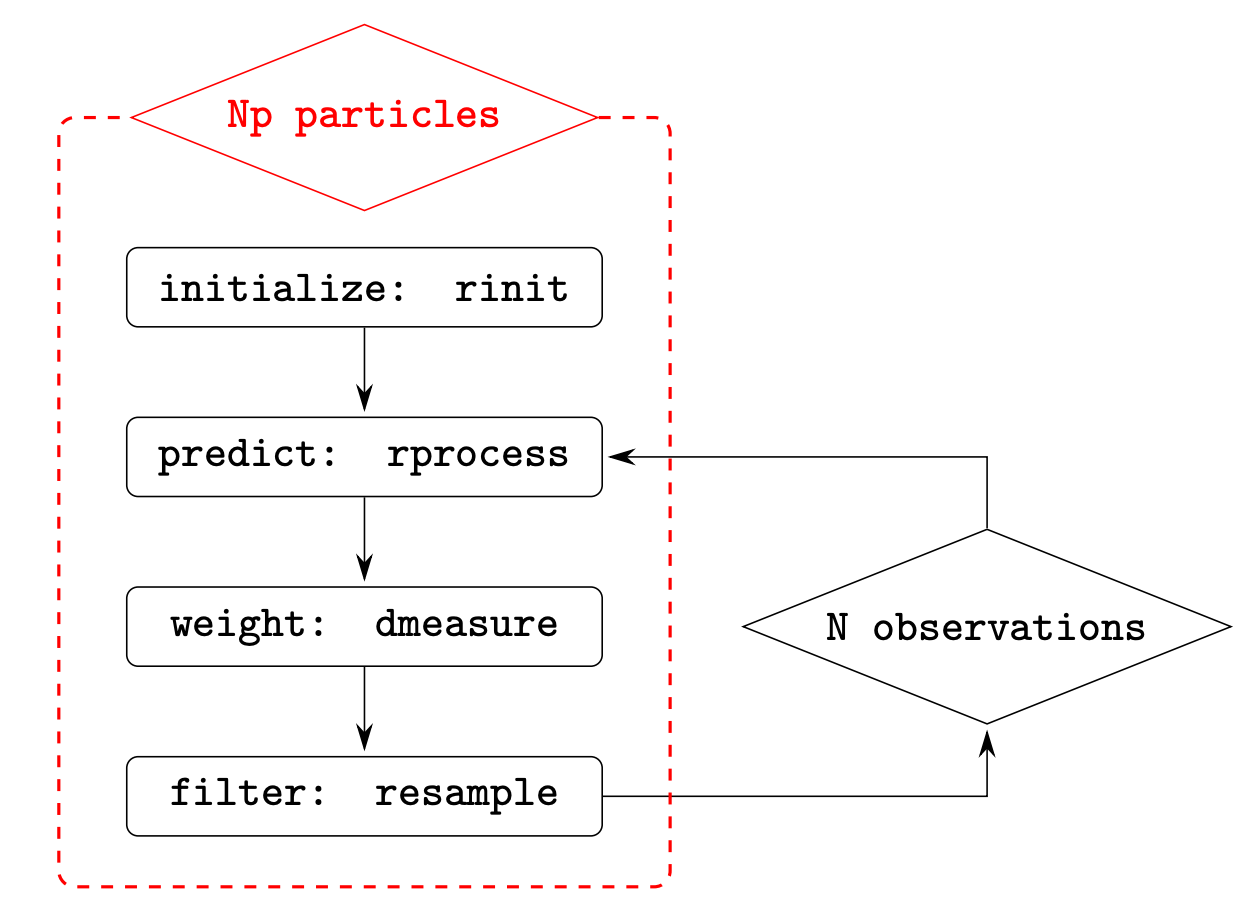
\includegraphics[height=6cm]{../graphics/lec3pf.png}
\end{center}

\hypertarget{parallel-computing}{%
\subsection{Parallel computing}\label{parallel-computing}}

It will be helpful to parallelize most of the computations. Most
machines nowadays have multiple cores and using this computational
capacity is as simple as:

\begin{enumerate}
\def\labelenumi{\arabic{enumi}.}
\tightlist
\item
  letting \texttt{R} know you plan to use multiple processors;
\item
  using the parallel for loop provided by the \texttt{foreach} package;
  and
\item
  paying proper attention to the use of parallel random number
  generators (RNG).
\end{enumerate}

For example:

\begin{Shaded}
\begin{Highlighting}[]
\FunctionTok{library}\NormalTok{(foreach)            }\CommentTok{\# load foreach}
\FunctionTok{library}\NormalTok{(doFuture)           }\CommentTok{\# load doFuture (and future)}
\FunctionTok{plan}\NormalTok{(multisession)          }\CommentTok{\# using multiple R sessions}
\end{Highlighting}
\end{Shaded}

The second line tells \texttt{foreach} that we will use the
\texttt{doFuture} backend. By default, R will attempt to determine how
many cores are available and will run an appropriate number of
concurrent R processes.

\hypertarget{particle-filtering-in-pomp}{%
\subsection{Particle filtering in
pomp}\label{particle-filtering-in-pomp}}

Recall the measles-outbreak example and the stochastic SIR model that we
construct in the previous lesson, we can using the \texttt{pfilter}
function to compute the likelihood using particle filtering method,
given the parameters chosen by looking at simulations. \texttt{R} code
to build the model is available \href{model_measSIR.R}{here}. We can
execute this code by sourcing the file and check the parameters:

\begin{Shaded}
\begin{Highlighting}[]
\FunctionTok{source}\NormalTok{(}\StringTok{"model\_measSIR.R"}\NormalTok{)}
\NormalTok{measSIR}\SpecialCharTok{@}\NormalTok{params}
\end{Highlighting}
\end{Shaded}

\begin{verbatim}
   Beta   Gamma     Rho       k     Eta       N 
1.5e+01 5.0e-01 5.0e-01 1.0e+01 6.0e-02 3.8e+04 
\end{verbatim}

\framebreak

In pomp, we can compute the likelihood using the particle filtering
method, implemented by function \texttt{pfilter}. The argument
\texttt{Np} assigns the number of particles used:

\begin{Shaded}
\begin{Highlighting}[]
\FunctionTok{library}\NormalTok{(pomp)}
\NormalTok{pf }\OtherTok{\textless{}{-}}\NormalTok{ measSIR }\SpecialCharTok{|\textgreater{}} \FunctionTok{pfilter}\NormalTok{(}\AttributeTok{Np=}\DecValTok{5000}\NormalTok{)}
\FunctionTok{logLik}\NormalTok{(pf)}
\end{Highlighting}
\end{Shaded}

\begin{verbatim}
[1] -131.0779
\end{verbatim}

\framebreak

The particle filtering method relies heavily on the state process and
the measurement model. Therefore, it is necessary to make sure that the
basic particle filter is working.

\begin{enumerate}
\def\labelenumi{\arabic{enumi}.}
\tightlist
\item
  Check the \texttt{rprocess} and the \texttt{rmeasure} by simulation,
  as shown in Lesson 2:
\end{enumerate}

\begin{Shaded}
\begin{Highlighting}[]
\NormalTok{measSIR }\SpecialCharTok{|\textgreater{}}
  \FunctionTok{simulate}\NormalTok{(}\AttributeTok{nsim=}\DecValTok{20}\NormalTok{,}\AttributeTok{format=}\StringTok{"data.frame"}\NormalTok{,}\AttributeTok{include.data=}\ConstantTok{TRUE}\NormalTok{) }\SpecialCharTok{|\textgreater{}}
  \FunctionTok{ggplot}\NormalTok{(}\FunctionTok{aes}\NormalTok{(}\AttributeTok{x=}\NormalTok{week,}\AttributeTok{y=}\NormalTok{reports,}\AttributeTok{group=}\NormalTok{.id,}\AttributeTok{color=}\NormalTok{.id}\SpecialCharTok{==}\StringTok{"data"}\NormalTok{)) }\SpecialCharTok{+}
  \FunctionTok{geom\_line}\NormalTok{() }\SpecialCharTok{+} \FunctionTok{guides}\NormalTok{(}\AttributeTok{color=}\StringTok{"none"}\NormalTok{)}
\end{Highlighting}
\end{Shaded}

\begin{figure}[h!]

{\centering 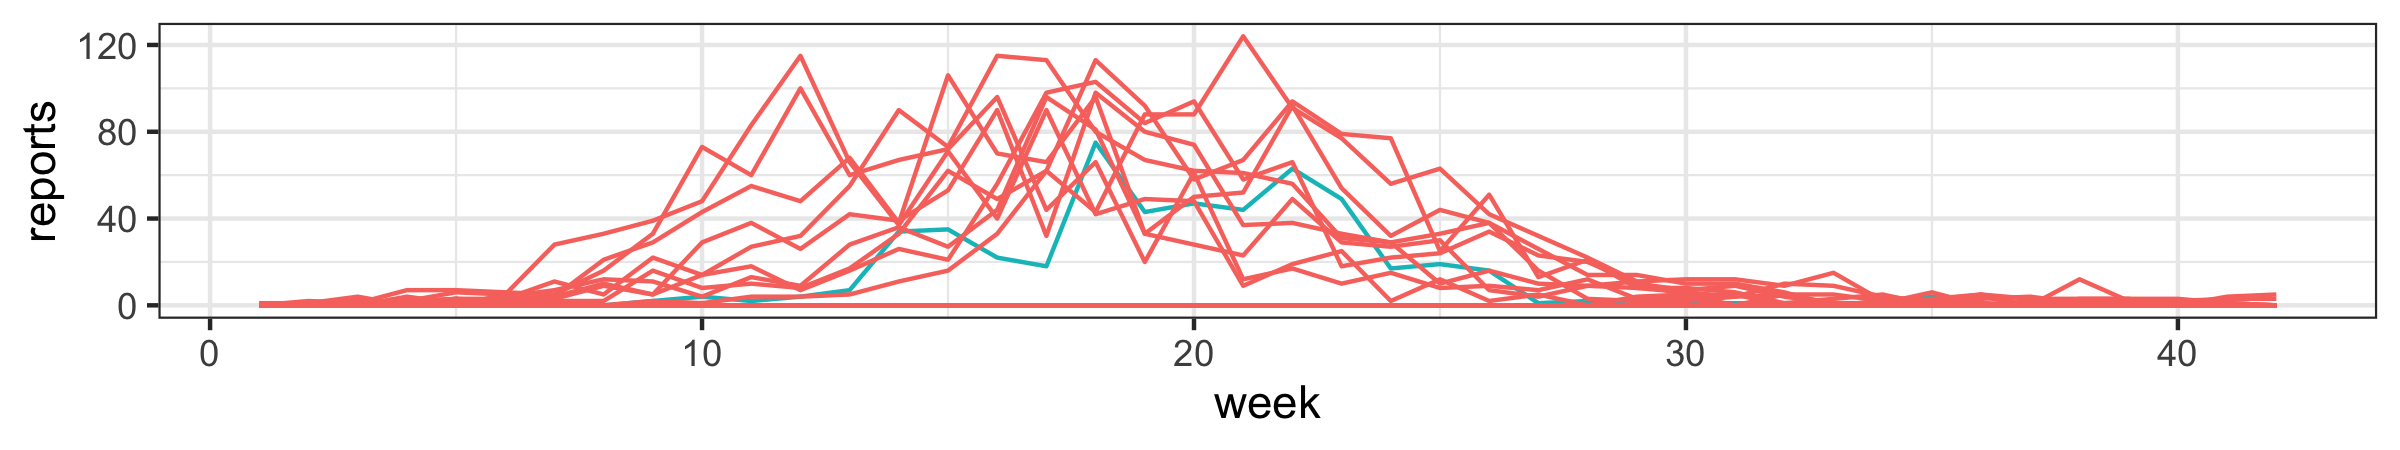
\includegraphics{tmp//figure/pf-diagnostic-1-1.png}

}

\end{figure}

\framebreak

\begin{enumerate}
\def\labelenumi{\arabic{enumi}.}
\setcounter{enumi}{1}
\tightlist
\item
  A diagnostic plot to check the \texttt{rprocess} and the
  \texttt{dmeasure}:
\end{enumerate}

\begin{Shaded}
\begin{Highlighting}[]
\FunctionTok{plot}\NormalTok{(pf)}
\end{Highlighting}
\end{Shaded}

\begin{itemize}
\item
  The data, \texttt{reports};
\item
  The \textbf{effective sample size} of the particle filter,
  \texttt{ess};
\item
  The log-likelihood of each observation conditioned on the preceding
  ones, \texttt{cond.logLik}.
\end{itemize}

\vspace{-10mm}

\begin{figure}[h!]

{\centering 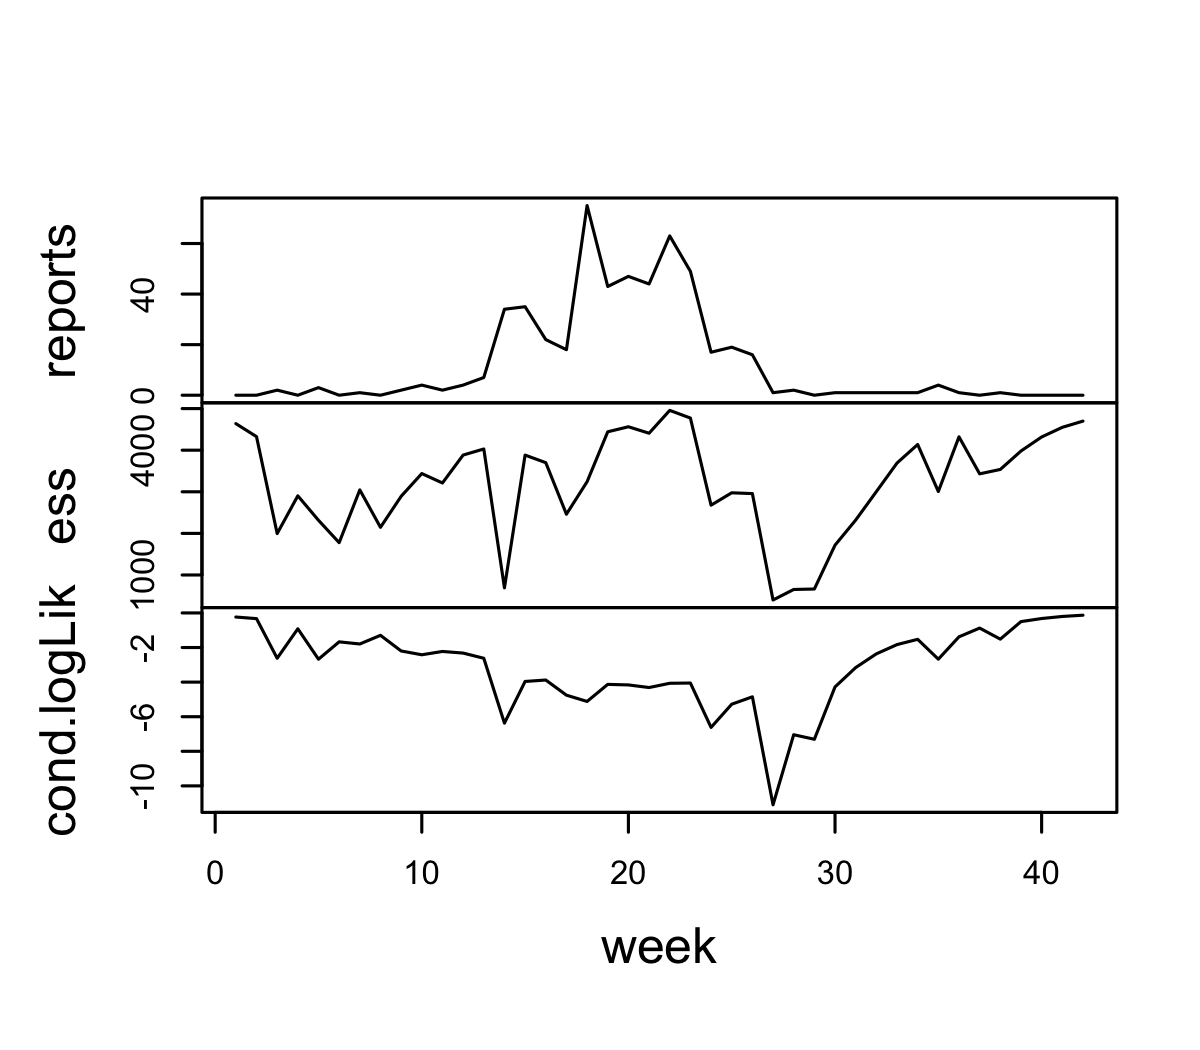
\includegraphics{tmp//figure/pf-diagnostic-2-2-1.png}

}

\end{figure}

\framebreak

\begin{enumerate}
\def\labelenumi{\arabic{enumi}.}
\setcounter{enumi}{2}
\tightlist
\item
  The Monte Carlo variability of the likelihood:
\end{enumerate}

\begin{Shaded}
\begin{Highlighting}[]
\FunctionTok{plan}\NormalTok{(multisession)}
\FunctionTok{foreach}\NormalTok{ (}
  \AttributeTok{i=}\DecValTok{1}\SpecialCharTok{:}\DecValTok{10}\NormalTok{, }\AttributeTok{.combine=}\NormalTok{c, }\AttributeTok{.options.future=}\FunctionTok{list}\NormalTok{(}\AttributeTok{seed=}\DecValTok{652643293}\NormalTok{)}
\NormalTok{) }\SpecialCharTok{\%dofuture\%}\NormalTok{ \{}
\NormalTok{    measSIR }\SpecialCharTok{|\textgreater{}} \FunctionTok{pfilter}\NormalTok{(}\AttributeTok{Np=}\DecValTok{5000}\NormalTok{)}
\NormalTok{\} }\OtherTok{{-}\textgreater{}}\NormalTok{ pf}
\FunctionTok{logLik}\NormalTok{(pf) }\OtherTok{{-}\textgreater{}}\NormalTok{ ll}
\FunctionTok{logmeanexp}\NormalTok{(ll,}\AttributeTok{se=}\ConstantTok{TRUE}\NormalTok{)}
\end{Highlighting}
\end{Shaded}

\begin{verbatim}
        est          se 
-130.037782    1.253115 
\end{verbatim}

Note that we set the parallel RNG seed in the \texttt{foreach} call.

\hypertarget{likelihood-based-inference}{%
\section{Likelihood-based inference}\label{likelihood-based-inference}}

\hypertarget{parameter-estimates-and-uncertainty-quantification}{%
\section{Parameter estimates and uncertainty
quantification}\label{parameter-estimates-and-uncertainty-quantification}}

\hypertarget{review-of-likelihood-based-inference}{%
\subsection{Review of likelihood-based
inference}\label{review-of-likelihood-based-inference}}

For now, let us suppose that software exists to evaluate and maximize
the likelihood function, up to a tolerable numerical error, for the
dynamic models of interest. Our immediate task is to think about how to
use that capability.

\begin{itemize}
\tightlist
\item
  Likelihood-based inference (meaning statistical tools based on the
  likelihood function) provides tools for parameter estimation, standard
  errors, hypothesis tests and diagnosing model misspecification.
\item
  Likelihood-based inference often (but not always) has favorable
  theoretical properties. Here, we are not especially concerned with the
  underlying theory of likelihood-based inference. On any practical
  problem, we can check the properties of a statistical procedure by
  simulation experiments.
\end{itemize}

\hypertarget{the-maximum-likelihood-estimate-mle}{%
\subsection{The maximum likelihood estimate
(MLE)}\label{the-maximum-likelihood-estimate-mle}}

\begin{itemize}
\tightlist
\item
  A maximum likelihood estimate (MLE) is \begin{equation*}
   \hat\theta = \argmax_{\theta} \loglik(\theta),
      \end{equation*} where \(\argmax_{\theta} g(\theta)\) means a value
  of argument \(\theta\) at which the maximum of the function \(g\) is
  attained, so
  \(g\left(\argmax_{\theta} g(\theta)\right) = \max_\theta g(\theta)\).
\item
  If there are many values of \(\theta\) giving the same maximum value
  of the likelihood, then an MLE still exists but is not unique.
\item
  Note that \(\argmax_{\theta} \lik(\theta)\) and
  \(\argmax_{\theta} \loglik(\theta)\) are the same. Why?
\end{itemize}

\hypertarget{standard-errors-for-the-mle}{%
\subsection{Standard errors for the
MLE}\label{standard-errors-for-the-mle}}

\begin{itemize}
\tightlist
\item
  Parameter estimates are not very useful without some measure of their
  uncertainty.
\item
  Usually, this means obtaining a confidence interval, or in practice an
  interval close to a true confidence interval which should formally be
  called an approximate confidence interval. In practice, the word
  ``approximate'' is often dropped!
\end{itemize}

There are three main approaches to estimating the statistical
uncertainty in an MLE.

\begin{enumerate}
\def\labelenumi{\arabic{enumi}.}
\item
  The Fisher information.
\item
  Profile likelihood estimation.
\item
  A simulation study, also known as a bootstrap.
\end{enumerate}

\hypertarget{fisher-information}{%
\subsection{Fisher information}\label{fisher-information}}

\begin{itemize}
\tightlist
\item
  A computationally quick approach when one has access to satisfactory
  numerical second derivatives of the log-likelihood.
\item
  The approximation is satisfactory only when \(\hat\theta\) is well
  approximated by a normal distribution.
\item
  Neither of the two requirements above are typically met for POMP
  models.
\item
  A review of standard errors via Fisher information is provided as a
  \href{fisherSE.html}{supplement}.
\end{itemize}

\hypertarget{profile-likelihood-estimation}{%
\subsection{Profile likelihood
estimation}\label{profile-likelihood-estimation}}

This approach is generally preferable to the Fisher information for POMP
models.

We will explain this method below and put it into practice in the
\href{https://kingaa.github.io/sbied/mif/}{next lesson}.

\hypertarget{the-bootstrap}{%
\subsection{The bootstrap}\label{the-bootstrap}}

\begin{itemize}
\tightlist
\item
  If done carefully and well, this can be the best approach.
\item
  A confidence interval is a claim about reproducibility. You claim, so
  far as your model is correct, that on 95\% of realizations from the
  model, a 95\% confidence interval you have constructed will cover the
  true value of the parameter.
\item
  A simulation study can check this claim fairly directly, but requires
  the most effort.
\item
  The simulation study takes time for you to develop and debug, time for
  you to explain, and time for the reader to understand and check what
  you have done. We usually carry out simulation studies to check our
  main conclusions only.
\item
  Further discussion of bootstrap methods for POMP models is provided as
  a \href{bootstrap.html}{supplement}.
\end{itemize}

\hypertarget{confidence-intervals-via-the-profile-likelihood}{%
\subsection{Confidence intervals via the profile
likelihood}\label{confidence-intervals-via-the-profile-likelihood}}

\begin{itemize}
\tightlist
\item
  Let's consider the problem of obtaining a confidence interval for the
  first component of \(\theta\). We'll write \[\theta=(\phi,\psi).\]
\item
  The \textbf{profile log-likelihood function} of \(\phi\) is defined to
  be \begin{equation*}
    \profileloglik{{}}(\phi) = \max_{\psi}\loglik(\phi,\psi).
  \end{equation*} In general, the profile likelihood of one parameter is
  constructed by maximizing the likelihood function over all other
  parameters.
\item
  Note that,
  \(\max_{\phi}\profileloglik{{}}(\phi) = \max_{\theta}\loglik(\theta)\)
  and that maximizing the profile likelihood
  \(\profileloglik{{}}(\phi)\) gives the MLE, \(\hat{\theta}\). Why?
\item
  An approximate 95\% confidence interval for \(\phi\) is given by
  \begin{equation*}
    \big\{\phi : \loglik(\hat\theta) - \profileloglik{{}}(\phi) < 1.92\big\}.
  \end{equation*}
\item
  This is known as a profile likelihood confidence interval. The cutoff
  \(1.92\) is derived using
  \href{https://en.wikipedia.org/wiki/Likelihood-ratio_test\#Distribution:_Wilks.27s_theorem}{Wilks'
  theorem}, which we will discuss in more detail when we develop
  likelihood ratio tests.
\item
  Although the asymptotic justification of Wilks' theorem is the same
  limit that justifies the Fisher information standard errors, profile
  likelihood confidence intervals tend to work better than Fisher
  information confidence intervals when \(N\) is not so
  large---particularly when the log-likelihood function is not close to
  quadratic near its maximum.
\end{itemize}

\hypertarget{geometry-of-the-likelihood-function}{%
\section{Geometry of the likelihood
function}\label{geometry-of-the-likelihood-function}}

\hypertarget{the-likelihood-surface}{%
\subsection{The likelihood surface}\label{the-likelihood-surface}}

\begin{itemize}
\tightlist
\item
  It is extremely useful to visualize the geometric surface defined by
  the likelihood function.
\item
  If \(\Theta\) is two-dimensional, then the surface \(\loglik(\theta)\)
  has features like a landscape.
\item
  Local maxima of \(\loglik(\theta)\) are peaks.
\item
  Local minima are valleys.
\item
  Peaks may be separated by a valley or may be joined by a ridge. If you
  go along the ridge, you may be able to go from one peak to the other
  without losing much elevation. Narrow ridges can be easy to fall off,
  and hard to get back on to.
\item
  In higher dimensions, one can still think of peaks and valleys and
  ridges. However, as the dimension increases it quickly becomes hard to
  imagine the surface.
\end{itemize}

\hypertarget{exploring-the-likelihood-surface-slices}{%
\subsection{Exploring the likelihood surface:
slices}\label{exploring-the-likelihood-surface-slices}}

\begin{itemize}
\item
  To get an idea of what the likelihood surface looks like in the
  neighborhood of a point in parameter space, we can construct some
  likelihood \emph{slices}.
\item
  A likelihood slice is a cross-section through the likelihood surface.
\item
  We'll make slices for our Consett measles POMP model, in the \(\beta\)
  and \(\mu_{IR}\) directions.
\item
  Both slices will pass through our current candidate parameter vector,
  stored in the \texttt{pomp} model object.
\end{itemize}

\vfill

\textbf{Questions}:

\begin{enumerate}
\def\labelenumi{\arabic{enumi}.}
\item
  What is the difference between a likelihood slice and a profile?
\item
  What is the consequence of this difference for the statistical
  interpretation of these plots?
\item
  How should you decide whether to compute a profile or a slice?
\end{enumerate}

\vspace{3mm}

\href{./Q_slice.html}{Worked solution to the Exercise}

\hypertarget{slicing-the-measles-sir-likelihood}{%
\subsection{Slicing the measles SIR
likelihood}\label{slicing-the-measles-sir-likelihood}}

\begin{itemize}
\tightlist
\item
  We first construct a data frame to explore the parameter slice, with
  \(40\times 3+40\times 3=240\) rows:
\end{itemize}

\begin{Shaded}
\begin{Highlighting}[]
\FunctionTok{slice\_design}\NormalTok{(}
  \AttributeTok{center =} \FunctionTok{coef}\NormalTok{(measSIR),}
  \AttributeTok{Beta =} \FunctionTok{rep}\NormalTok{(}\FunctionTok{seq}\NormalTok{(}\AttributeTok{from=}\DecValTok{5}\NormalTok{,}\AttributeTok{to=}\DecValTok{30}\NormalTok{,}\AttributeTok{length=}\DecValTok{40}\NormalTok{),}\AttributeTok{each=}\DecValTok{3}\NormalTok{),}
  \AttributeTok{Gamma =} \FunctionTok{rep}\NormalTok{(}\FunctionTok{seq}\NormalTok{(}\AttributeTok{from=}\FloatTok{0.2}\NormalTok{,}\AttributeTok{to=}\DecValTok{2}\NormalTok{,}\AttributeTok{length=}\DecValTok{40}\NormalTok{),}\AttributeTok{each=}\DecValTok{3}\NormalTok{)}
\NormalTok{) }\OtherTok{{-}\textgreater{}}\NormalTok{ param\_slice}

\FunctionTok{dim}\NormalTok{(param\_slice)}
\end{Highlighting}
\end{Shaded}

\begin{verbatim}
[1] 240   7
\end{verbatim}

\framebreak

\begin{itemize}
\tightlist
\item
  We compute the likelihoods \(3\) times for each combination (i.e.,
  row) in \texttt{param\_slice}:
\end{itemize}

\begin{Shaded}
\begin{Highlighting}[]
\FunctionTok{library}\NormalTok{(iterators)}
\FunctionTok{plan}\NormalTok{(multisession)}
\FunctionTok{foreach}\NormalTok{ (}\AttributeTok{theta=}\FunctionTok{iter}\NormalTok{(param\_slice,}\StringTok{"row"}\NormalTok{), }\AttributeTok{.combine=}\NormalTok{rbind, }
  \AttributeTok{.options.future=}\FunctionTok{list}\NormalTok{(}\AttributeTok{seed=}\DecValTok{108028909}\NormalTok{)) }\SpecialCharTok{\%dofuture\%}\NormalTok{ \{}
\NormalTok{  measSIR }\SpecialCharTok{|\textgreater{}} \FunctionTok{pfilter}\NormalTok{(}\AttributeTok{params=}\NormalTok{theta,}\AttributeTok{Np=}\DecValTok{5000}\NormalTok{) }\OtherTok{{-}\textgreater{}}\NormalTok{ pf}
\NormalTok{  theta}\SpecialCharTok{$}\NormalTok{loglik }\OtherTok{\textless{}{-}} \FunctionTok{logLik}\NormalTok{(pf)}
\NormalTok{  theta}
\NormalTok{\} }\OtherTok{{-}\textgreater{}}\NormalTok{ lik\_slice}
\end{Highlighting}
\end{Shaded}

\framebreak

\begin{figure}[h!]

{\centering 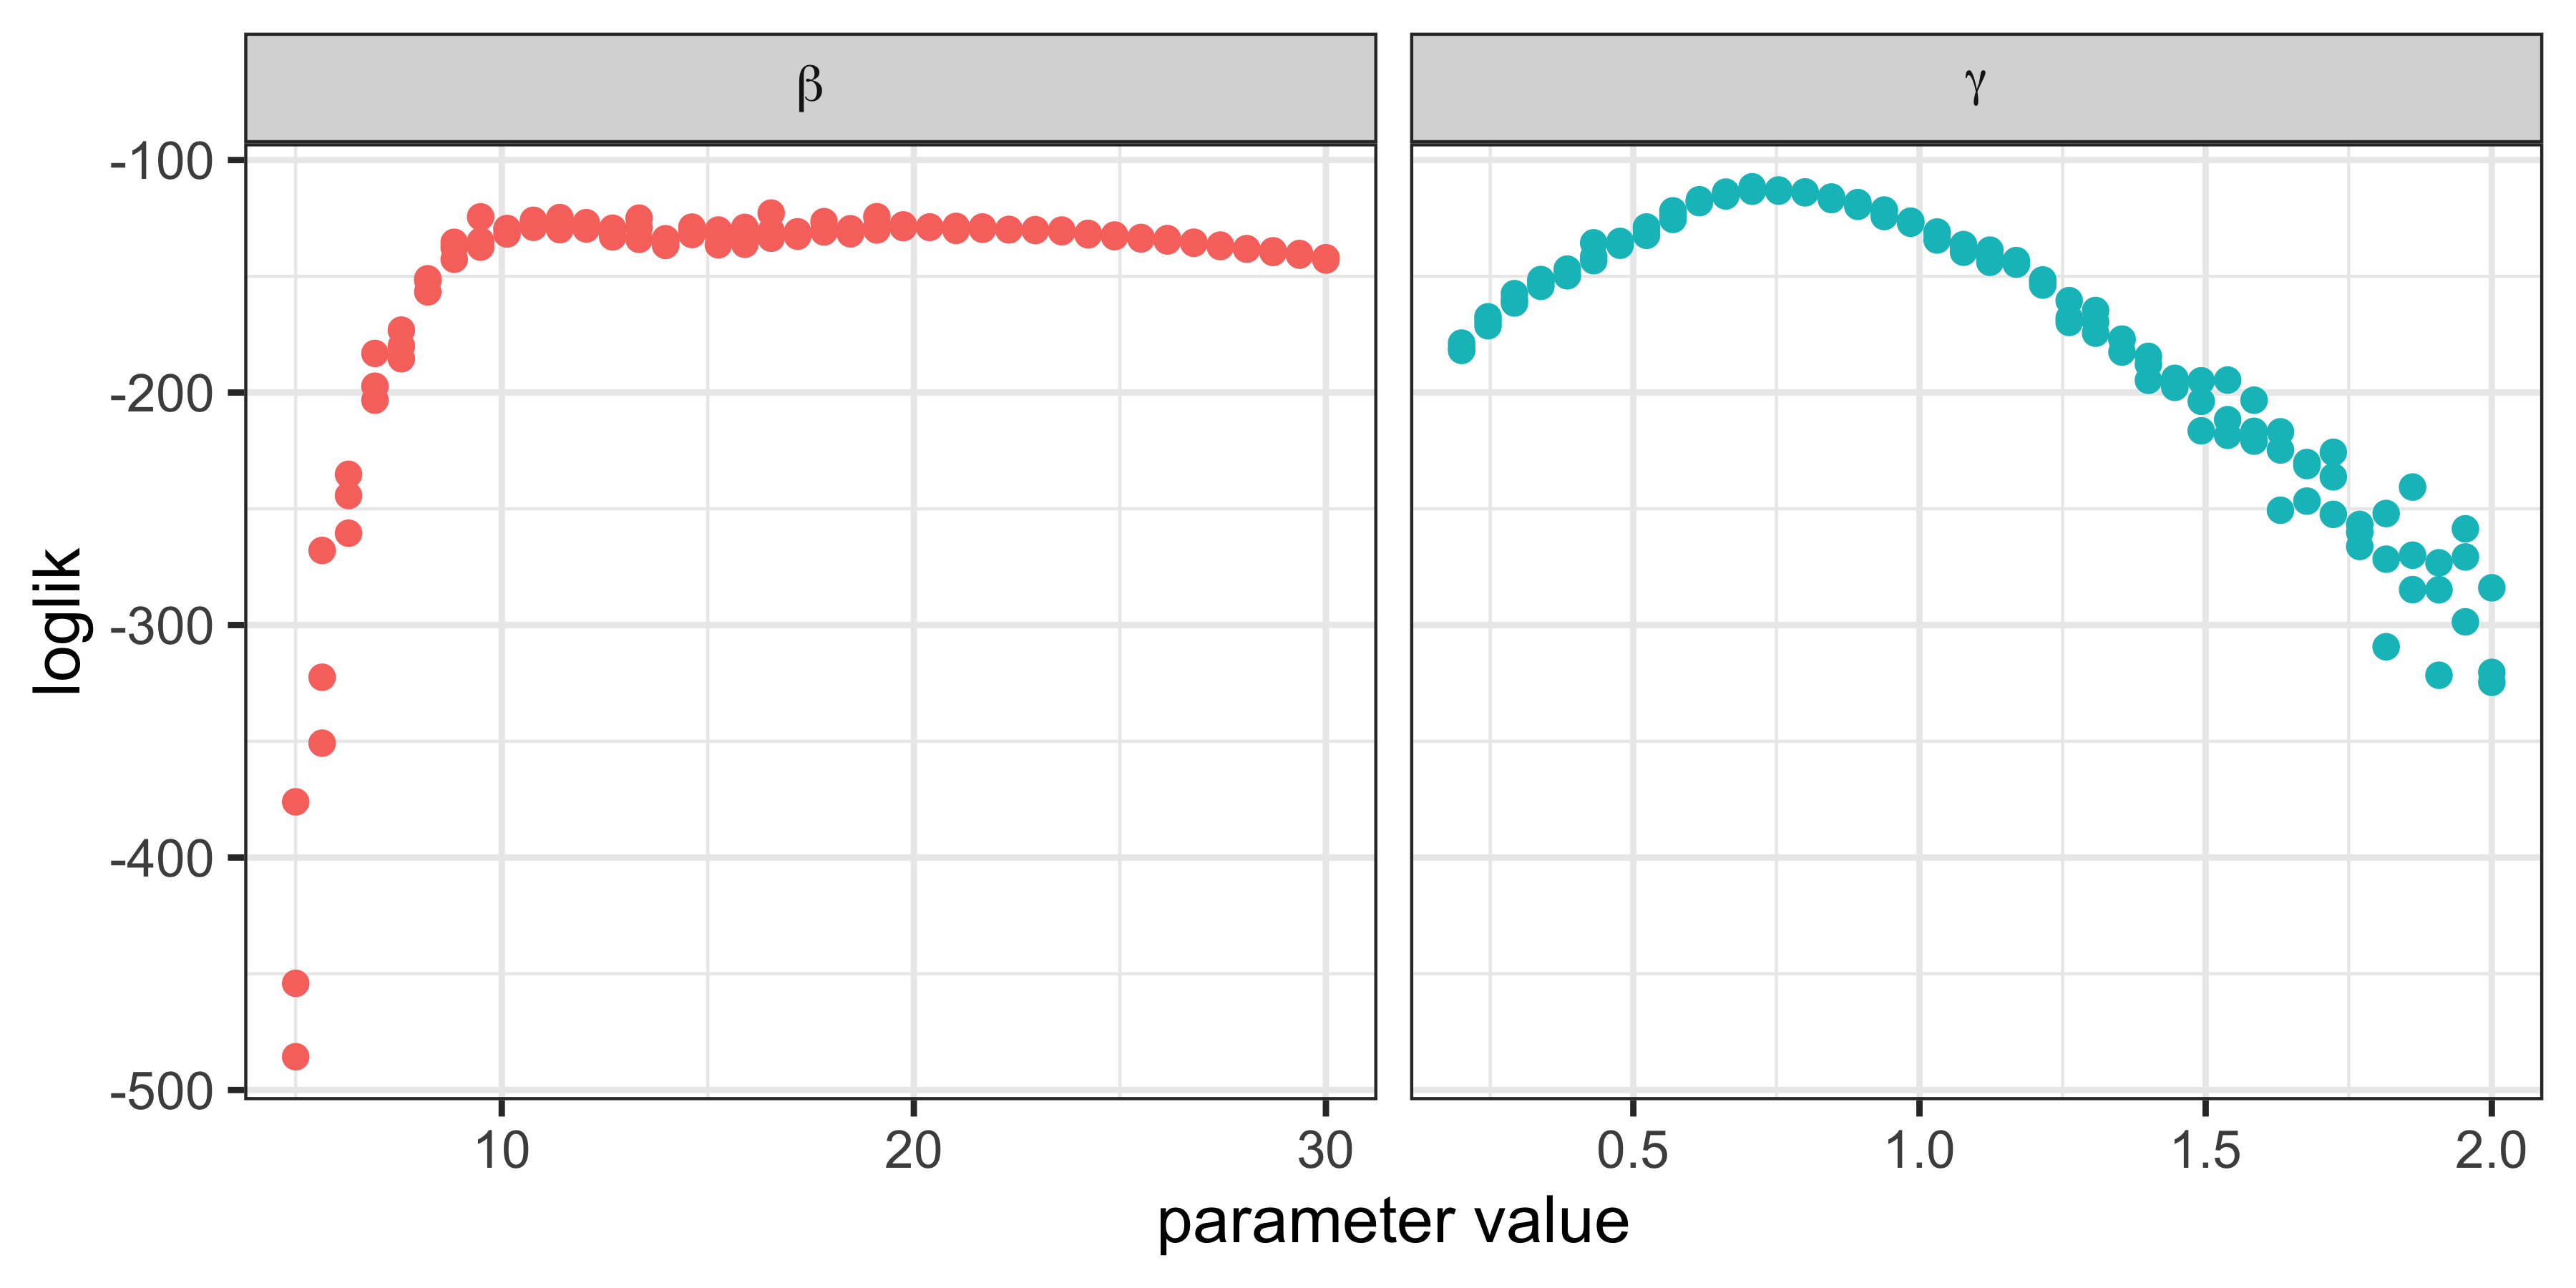
\includegraphics[width=5in,height=2in]{tmp//figure/like-slice-plot-1.png}

}

\end{figure}

\begin{itemize}
\tightlist
\item
  Slices offer a very limited perspective on the geometry of the
  likelihood surface.
\item
  When there are only one or two unknown parameters, we can evaluate the
  likelihood at a grid of points and visualize the surface directly.
\end{itemize}

\hypertarget{two-dimensional-likelihood-slice}{%
\subsection{Two-dimensional likelihood
slice}\label{two-dimensional-likelihood-slice}}

\begin{itemize}
\tightlist
\item
  We first construct the parameters grid data frame
  \texttt{param\_grid}, with \(40\times 3 \times 40\times 3=14,400\)
  rows:
\end{itemize}

\begin{Shaded}
\begin{Highlighting}[]
\FunctionTok{expand.grid}\NormalTok{(}
  \AttributeTok{Beta =} \FunctionTok{rep}\NormalTok{(}\FunctionTok{seq}\NormalTok{(}\AttributeTok{from=}\DecValTok{10}\NormalTok{,}\AttributeTok{to=}\DecValTok{30}\NormalTok{,}\AttributeTok{length=}\DecValTok{40}\NormalTok{), }\AttributeTok{each=}\DecValTok{3}\NormalTok{),}
  \AttributeTok{Gamma =} \FunctionTok{rep}\NormalTok{(}\FunctionTok{seq}\NormalTok{(}\AttributeTok{from=}\FloatTok{0.4}\NormalTok{,}\AttributeTok{to=}\FloatTok{1.5}\NormalTok{,}\AttributeTok{length=}\DecValTok{40}\NormalTok{), }\AttributeTok{each=}\DecValTok{3}\NormalTok{),}
  \AttributeTok{Rho =} \FloatTok{0.5}\NormalTok{, }\AttributeTok{k=}\DecValTok{10}\NormalTok{, }\AttributeTok{Eta=}\FloatTok{0.06}\NormalTok{, }\AttributeTok{N=}\DecValTok{38000}
\NormalTok{) }\OtherTok{{-}\textgreater{}}\NormalTok{ param\_grid}

\FunctionTok{dim}\NormalTok{(param\_grid)}
\end{Highlighting}
\end{Shaded}

\begin{verbatim}
[1] 14400     6
\end{verbatim}

\framebreak

\begin{itemize}
\tightlist
\item
  We then compute likelihoods for each of the combinations:
\end{itemize}

\begin{Shaded}
\begin{Highlighting}[]
\FunctionTok{plan}\NormalTok{(multisession)}
\FunctionTok{foreach}\NormalTok{ (}\AttributeTok{theta=}\FunctionTok{iter}\NormalTok{(param\_grid,}\StringTok{"row"}\NormalTok{), }\AttributeTok{.combine=}\NormalTok{rbind,}
  \AttributeTok{.options.future=}\FunctionTok{list}\NormalTok{(}\AttributeTok{seed=}\DecValTok{421776444}\NormalTok{)) }\SpecialCharTok{\%dofuture\%}\NormalTok{ \{}
\NormalTok{  measSIR }\SpecialCharTok{|\textgreater{}} \FunctionTok{pfilter}\NormalTok{(}\AttributeTok{params=}\NormalTok{theta,}\AttributeTok{Np=}\DecValTok{5000}\NormalTok{) }\OtherTok{{-}\textgreater{}}\NormalTok{ pf}
\NormalTok{  theta}\SpecialCharTok{$}\NormalTok{loglik }\OtherTok{\textless{}{-}} \FunctionTok{logLik}\NormalTok{(pf)}
\NormalTok{  theta}
\NormalTok{\} }\OtherTok{{-}\textgreater{}}\NormalTok{ lik\_grid}
\end{Highlighting}
\end{Shaded}

\framebreak

\begin{figure}[h!]

{\centering 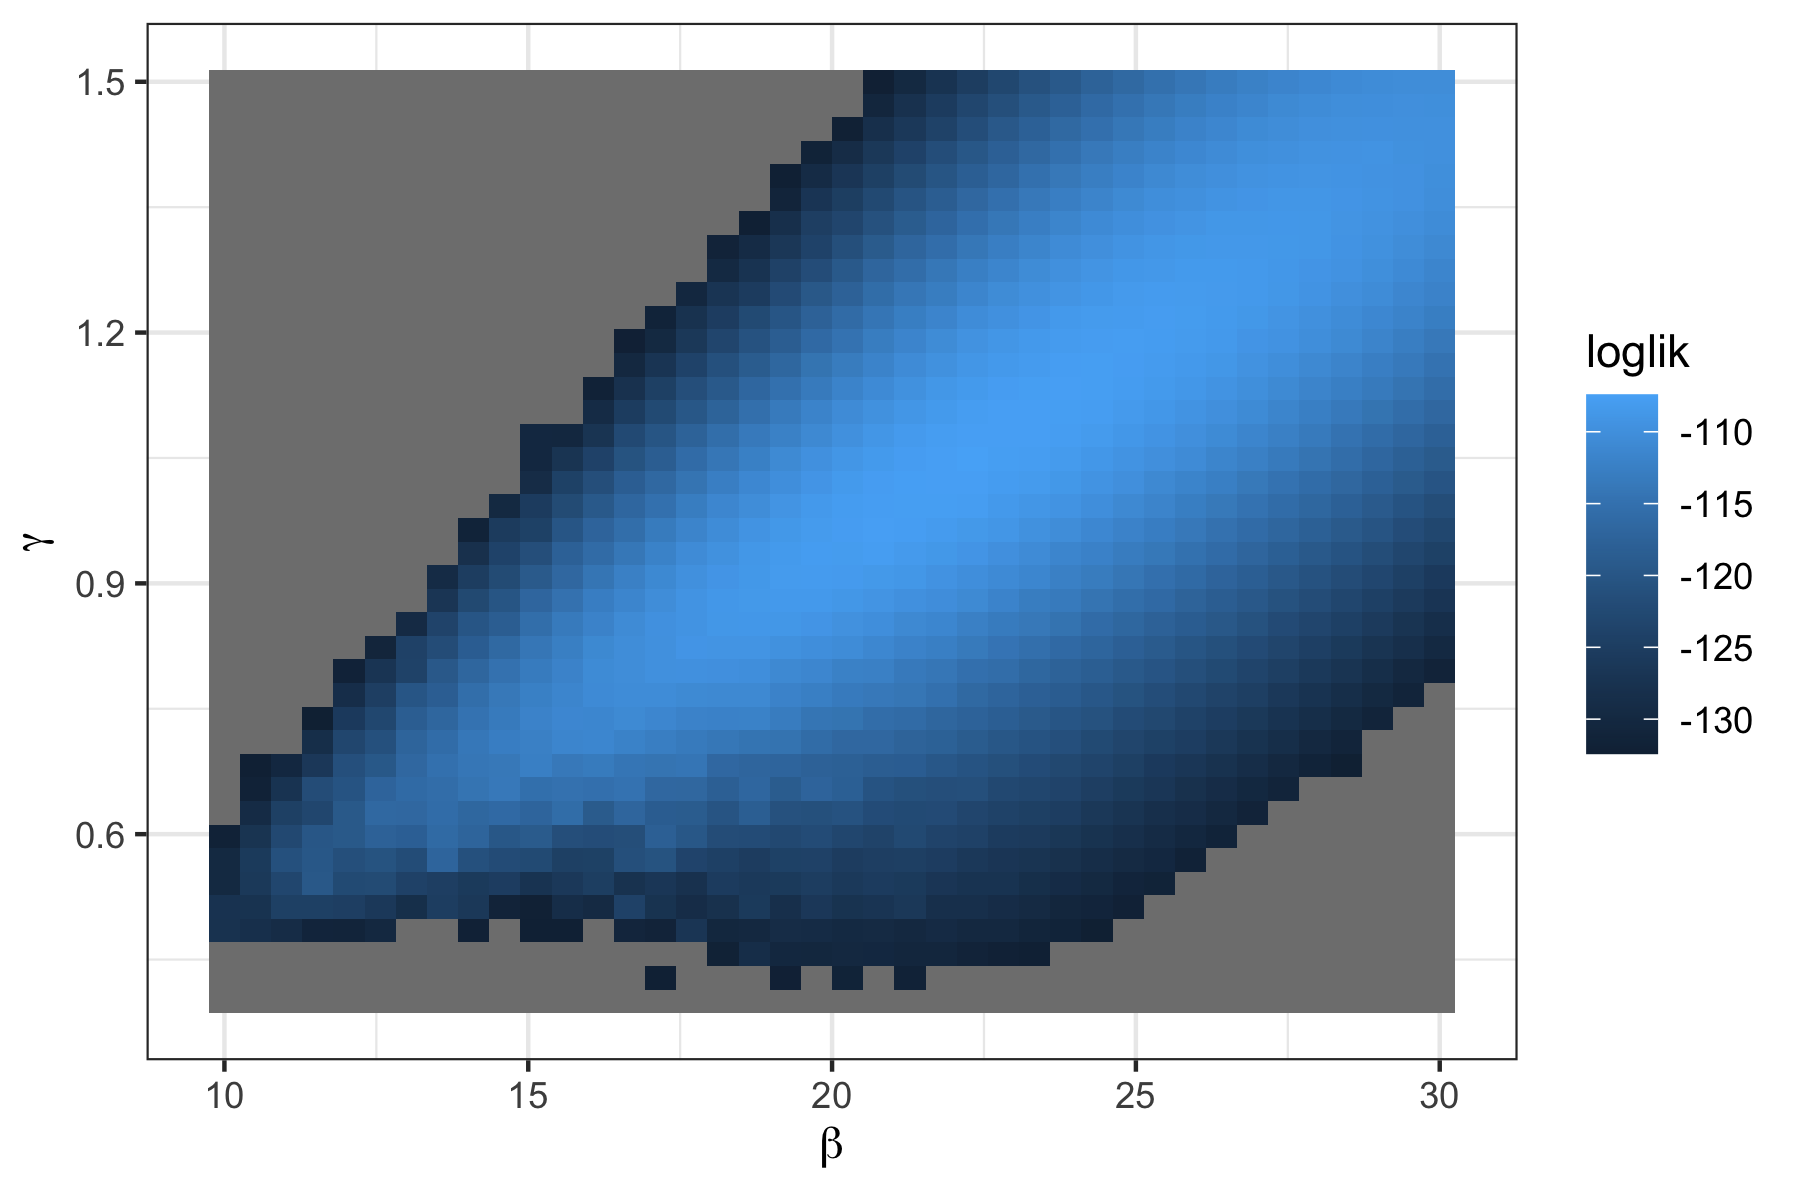
\includegraphics[width=4.8in,height=3.2in]{tmp//figure/pfilter-grid1-plot-1.png}

}

\end{figure}

\framebreak

In the above, all points with log-likelihoods less than 25 units below
the maximum are shown in grey.

\begin{itemize}
\item
  Notice some features of the log-likelihood surface, and its estimate
  from the particle filter, that can cause difficulties for numerical
  methods:

  \begin{enumerate}
  \def\labelenumi{\arabic{enumi}.}
  \tightlist
  \item
    The surface is wedge-shaped, so its curvature varies considerably.
    By contrast, asymptotic theory predicts a parabolic surface that has
    constant curvature.
  \item
    Monte Carlo noise in the likelihood evaluation makes it hard to pick
    out exactly where the likelihood is maximized. Nevertheless, the
    major features of the likelihood surface are evident despite the
    noise.
  \end{enumerate}
\item
  Wedge-shaped relationships between parameters, and nonlinear
  relationships, are common features of epidemiological dynamic models.
  We'll see this in the case studies.
\end{itemize}

\hypertarget{exercises}{%
\section{Exercises}\label{exercises}}

\hypertarget{cost-of-a-particle-filter-calculation}{%
\subsection{Cost of a particle-filter
calculation}\label{cost-of-a-particle-filter-calculation}}

\begin{itemize}
\tightlist
\item
  How much computer processing time does a particle filter take?
\item
  How does this scale with the number of particles?
\end{itemize}

Form a conjecture based upon your understanding of the algorithm. Test
your conjecture by running a sequence of particle filter operations,
with increasing numbers of particles (\texttt{Np}), measuring the time
taken for each one using \texttt{system.time}. Plot and interpret your
results.

\vfill

\href{./expense.html}{Worked solution to the Exercise}

\hypertarget{log-likelihood-estimation}{%
\subsection{log-likelihood estimation}\label{log-likelihood-estimation}}

Here are some desiderata for a Monte Carlo log-likelihood approximation:

\begin{itemize}
\tightlist
\item
  It should have low Monte Carlo bias and variance.
\item
  It should be presented together with estimates of the bias and
  variance so that we know the extent of Monte Carlo uncertainty in our
  results.
\item
  It should be computed in a length of time appropriate for the
  circumstances.
\end{itemize}

Set up a likelihood evaluation for the measles model, choosing the
numbers of particles and replications so that your evaluation takes
approximately one minute on your machine.

\begin{itemize}
\tightlist
\item
  Provide a Monte Carlo standard error for your estimate.
\item
  Comment on the bias of your estimate.
\item
  Use doFuture to take advantage of multiple cores on your computer to
  improve your estimate.
\end{itemize}

\href{./loglikest.html}{Worked solution to the Exercise}

\hypertarget{exercises-1}{%
\subsection{Exercises}\label{exercises-1}}

\begin{enumerate}
\def\labelenumi{\arabic{enumi}.}
\item
  \textbf{One-dimensional likelihood slice}: Compute several likelihood
  slices in the \(\eta\) direction.
\item
  \textbf{Two-dimensional likelihood slice}: Compute a slice of the
  likelihood in the \(\beta\)-\(\eta\) plane.
\end{enumerate}

\hypertarget{more-on-likelihood-based-inference}{%
\section{More on likelihood-based
inference}\label{more-on-likelihood-based-inference}}

\hypertarget{maximizing-the-likelihood}{%
\section{Maximizing the likelihood}\label{maximizing-the-likelihood}}

\hypertarget{maximizing-the-particle-filter-likelihood}{%
\subsection{Maximizing the particle filter
likelihood}\label{maximizing-the-particle-filter-likelihood}}

\begin{itemize}
\tightlist
\item
  Likelihood maximization is key to profile intervals, likelihood ratio
  tests and AIC as well as the computation of the MLE.
\item
  An initial approach to likelihood maximization might be to stick the
  particle filter log-likelihood estimate into a standard numerical
  optimizer, such as the Nelder-Mead algorithm.
\item
  In practice this approach is unsatisfactory on all but the smallest
  POMP models. Standard numerical optimizers are not designed to
  maximize noisy and computationally expensive Monte Carlo functions.
\item
  Further investigation into this approach is available as a
  \href{pf-in-Nelder-Mead.html}{supplement}.
\item
  We'll present an \emph{iterated filtering algorithm} for maximizing
  the likelihood in a way that takes advantage of the structure of POMP
  models and the particle filter.
\item
  First, let's think a bit about some practical considerations in
  interpreting the MLE for a POMP.
\end{itemize}

\hypertarget{likelihood-based-model-selection-and-model-diagnostics}{%
\subsection{Likelihood-based model selection and model
diagnostics}\label{likelihood-based-model-selection-and-model-diagnostics}}

\begin{itemize}
\tightlist
\item
  For nested hypotheses, we can carry out model selection by likelihood
  ratio tests.
\item
  For non-nested hypotheses, likelihoods can be compared using Akaike's
  information criterion (AIC) or related methods.
\end{itemize}

\hypertarget{likelihood-ratio-test}{%
\section{Likelihood ratio test}\label{likelihood-ratio-test}}

\hypertarget{likelihood-ratio-tests-for-nested-hypotheses}{%
\subsection{Likelihood ratio tests for nested
hypotheses}\label{likelihood-ratio-tests-for-nested-hypotheses}}

\begin{itemize}
\tightlist
\item
  The whole parameter space on which the model is defined is
  \(\Theta\subset\R^D\).
\item
  Suppose we have two \textbf{nested} hypotheses \begin{equation*}
    \begin{aligned}
      H^{\langle 0\rangle} &: \theta\in \Theta^{\langle 0\rangle}, \\
      H^{\langle 1\rangle} &: \theta\in \Theta^{\langle 1\rangle},
    \end{aligned}
  \end{equation*} defined via two nested parameter subspaces,
  \(\Theta^{\langle 0\rangle}\subset \Theta^{\langle 1\rangle}\), with
  respective dimensions
  \(D^{\langle 0\rangle}< D^{\langle 1\rangle}\le D\).
\item
  We consider the log-likelihood maximized over each of the hypotheses,
  \[
    \begin{aligned}
      \ell^{\langle 0\rangle} &= \sup_{\theta\in \Theta^{\langle 0\rangle}} \ell(\theta), \\
      \ell^{\langle 1\rangle} &= \sup_{\theta\in \Theta^{\langle 1\rangle}} \ell(\theta).
    \end{aligned}
  \]
\item
  \textbf{Wilks approximation}: under the hypothesis
  \(H^{\langle 0\rangle}\), \[
    \ell^{\langle 1\rangle} - \ell^{\langle 0\rangle} \approx \tfrac{1}{2}\,\chi^2_{D^{\langle 1\rangle}- D^{\langle 0\rangle}},
  \] where \(\chi^2_d\) is a chi-squared random variable on \(d\)
  degrees of freedom and \(\approx\) means ``is approximately
  distributed as''.
\item
  The Wilks approximation can be used to construct a hypothesis test of
  the null hypothesis \(H^{\langle 0\rangle}\) against the alternative
  \(H^{\langle 1\rangle}\).
\item
  This is called a \textbf{likelihood ratio test} since a difference of
  log-likelihoods corresponds to a ratio of likelihoods.
\item
  When the data are IID, \(N\to\infty\), and the hypotheses satisfy
  suitable regularity conditions, this approximation can be derived
  mathematically and is known as \textbf{Wilks' theorem}.
\item
  The chi-squared approximation to the likelihood ratio statistic may be
  useful, and can be assessed empirically by a simulation study, even in
  situations that do not formally satisfy any known theorem.
\end{itemize}

\hypertarget{wilks-theorem-and-profile-likelihood}{%
\subsection{Wilks' theorem and profile
likelihood}\label{wilks-theorem-and-profile-likelihood}}

\begin{itemize}
\tightlist
\item
  Suppose we have an MLE, written \(\hat\theta=(\hat\phi,\hat\psi)\),
  and a profile log-likelihood for \(\phi\), given by
  \(\profileloglik{{}}(\phi)\).
\item
  Consider the likelihood ratio test for the nested hypotheses
  \begin{equation*}
    \begin{aligned}
      H^{\langle 0\rangle} &: \phi = \phi_0, \\
      H^{\langle 1\rangle} &: \text{$\phi$ unconstrained}.
    \end{aligned}
  \end{equation*}
\item
  We can compute the 95\%-ile for a chi-squared distribution with one
  degree of freedom: \texttt{qchisq(0.95,df=1)}\(=3.841\).
\item
  Wilks' theorem then gives us a hypothesis test with approximate size
  \(5\%\) that rejects \(H^{\langle 0\rangle}\) if
  \(\profileloglik{{}}(\hat\phi)-\profileloglik{{}}(\phi_0)<3.84/2\).
\item
  It follows that, with probability \(95\%\), the true value of \(\phi\)
  falls in the set \begin{equation*}
    \big\{\phi: \profileloglik{{}}(\hat\phi)-\profileloglik{{}}(\phi)<1.92\big\}.
  \end{equation*} So, we have constructed a profile likelihood
  confidence interval, consisting of the set of points on the profile
  likelihood within \(1.92\) log units of the maximum.
\item
  This is an example of
  \href{https://www.stat.nus.edu.sg/~wloh/lecture17.pdf}{a general
  duality between confidence intervals and hypothesis tests}.
\end{itemize}

\hypertarget{information-criteria}{%
\section{Information criteria}\label{information-criteria}}

\hypertarget{akaikes-information-criterion-aic}{%
\subsection{Akaike's information criterion
(AIC)}\label{akaikes-information-criterion-aic}}

\begin{itemize}
\tightlist
\item
  Likelihood ratio tests provide an approach to model selection for
  nested hypotheses, but what do we do when models are not nested?
\item
  A more general approach is to compare likelihoods of different models
  by penalizing the likelihood of each model by a measure of its
  complexity.
\item
  Akaike's information criterion \textbf{AIC} is given by
  \begin{equation*}
    \mathrm{AIC} = -2\,\loglik(\hat{\theta}) + 2\,D
  \end{equation*} ``Minus twice the maximized log-likelihood plus twice
  the number of parameters.''
\item
  We are invited to select the model with the lowest AIC score.
\item
  AIC was derived as an approach to minimizing prediction error.
  Increasing the number of parameters leads to additional
  \textbf{overfitting} which can decrease predictive skill of the fitted
  model.
\item
  Viewed as a hypothesis test, AIC may have weak statistical properties.
  It can be a mistake to interpret AIC by making a claim that the
  favored model has been shown to provide a superior explanation of the
  data. However, viewed as a way to select a model with reasonable
  predictive skill from a range of possibilities, it is often useful.
\item
  AIC does not penalize model complexity beyond the consequence of
  reduced predictive skill due to overfitting. One can penalize
  complexity by incorporating a more severe penalty than the \(2D\) term
  above, such as via
  \href{https://en.wikipedia.org/wiki/Bayesian_information_criterion}{BIC}.
\item
  A practical approach is to use AIC, while taking care to view it as a
  procedure to select a reasonable predictive model and not as a formal
  hypothesis test.
\end{itemize}

\hypertarget{references}{%
\section{References}\label{references}}

\hypertarget{references-1}{%
\subsection{References}\label{references-1}}

\small

\hypertarget{refs}{}
\begin{CSLReferences}{1}{0}
\leavevmode\vadjust pre{\hypertarget{ref-Arulampalam2002}{}}%
Arulampalam, M. S., S. Maskell, N. Gordon, and T. Clapp. 2002. {``A
Tutorial on Particle Filters for Online Nonlinear, Non-{Gaussian}
{Bayesian} Tracking.''} \emph{IEEE Trans Signal Process} 50: 174--88.
\url{https://doi.org/10.1109/78.978374}.

\leavevmode\vadjust pre{\hypertarget{ref-Doucet2001}{}}%
Doucet, Arnaud, Nando de Freitas, and Neil Gordon, eds. 2001.
\emph{Sequential {Monte} {Carlo} Methods in Practice}. New York:
Springer-Verlag.

\leavevmode\vadjust pre{\hypertarget{ref-Fisher1922}{}}%
Fisher, R. A. 1922. {``On the Mathematical Foundations of Theoretical
Statistics.''} \emph{Philos Trans R Soc London A} 222: 309--68.
\url{https://doi.org/10.1098/rsta.1922.0009}.

\leavevmode\vadjust pre{\hypertarget{ref-King2016}{}}%
King, Aaron A., Dao Nguyen, and Edward L. Ionides. 2016. {``Statistical
Inference for Partially Observed {Markov} Processes via the {R} Package
Pomp.''} \emph{J Stat Softw} 69 (12): 1--43.
\url{https://doi.org/10.18637/jss.v069.i12}.

\leavevmode\vadjust pre{\hypertarget{ref-Kitagawa1987}{}}%
Kitagawa, Genshiro. 1987. {``Non-{Gauss}ian State-Space Modeling of
Nonstationary Time Series.''} \emph{J Am Stat Assoc} 82 (400): 1032--41.
\url{https://doi.org/10.1080/01621459.1987.10478534}.

\leavevmode\vadjust pre{\hypertarget{ref-Pawitan2001}{}}%
Pawitan, Yudi. 2001. \emph{{I}n {A}ll {L}ikelihood: {S}tatistical
{M}odelling and {I}nference {U}sing {L}ikelihood}. Oxford: Clarendon
Press.

\end{CSLReferences}

\hypertarget{license-acknowledgments-and-links}{%
\subsection{License, acknowledgments, and
links}\label{license-acknowledgments-and-links}}

\begin{itemize}
\item
  This lesson is prepared for the
  \href{https://kingaa.github.io/sbied/}{Simulation-based Inference for
  Epidemiological Dynamics} module at the Summer Institute in Statistics
  and Modeling in Infectious Diseases,
  \href{https://www.biostat.washington.edu/suminst/sismid}{SISMID}.
\item
  The materials build on \href{../acknowledge.html}{previous versions of
  this course and related courses}.
\item
  Licensed under the
  \href{https://creativecommons.org/licenses/by-nc/4.0/}{Creative
  Commons Attribution-NonCommercial license}. Please share and remix
  non-commercially, mentioning its origin.
  
\includegraphics[height=12pt]{../graphics/cc-by-nc}
\item
  Produced with R version 4.3.2 and pomp version 5.10.
\item
  Compiled on 2024-07-11.
\end{itemize}

\href{index.html}{Back to Lesson}

\href{./main.R}{\texttt{R} codes for this lesson}



\end{document}
